\documentclass[journal]{IEEEtran}

\usepackage{manuscript}

\title{CertGraph: Issuer-Scoped Certificate Provenance for Active Directory Certificate Services Investigation and Remediation}

\author{Md.~Hasan~Shahriar, Taufiq~Biswas, and Md.~Ramim~Hossain%
\thanks{The authors are with the Department of Electronics and Communication Engineering, Hajee Mohammad Danesh Science and Technology University (HSTU), Dinajpur-5200, Bangladesh. Corresponding author: Md. Hasan Shahriar (e-mail: hasanshahriar32@gmail.com).}}

\begin{document}

\maketitle

\begin{abstract}
Certificate-template restoration can hide the configuration that enabled an earlier Active Directory Certificate Services (ADCS) issuance while leaving the certificate usable. CertGraph reconstructs issuance-to-authentication links through an issuer-scoped evidence contract. It retains compatible candidates when identifiers are incomplete, distinguishes possible from definite attribution, and revises conclusions when evidence conflicts. A frozen study of 5,400 synthetic histories includes 2,000 randomized histories in which the contract retains 99.06\% of true observed links as candidates and resolves 55.82\% definitively. Four controlled Windows intervention matrices and a concurrent forest workload provide 72 certificate cases: 66 successful exact-certificate authentications, including 13 administrative uses, and six certificate-bound rejections. Fixed signed requests isolate the tested template-bit contrast, while current-patch controls distinguish UPN-only rejection from administrative use of SID-URL certificates after restoration. A guarded SQLite implementation agrees with the identity reference at all 5,423 evaluated prefixes. Budgeted sequential interdiction supplies a complementary remediation analysis on 120 graph/budget instances, with explicit small-instance optimality gaps. An auxiliary graph-learning study finds identical additive and bilinear classifications and misses every tested long-path positive. The evidence supports certificate-specific investigation in controlled laboratories and identifies the collection, source-trust and deployment conditions requiring further validation.
\end{abstract}

\begin{IEEEkeywords}
Active Directory security, certificate services, provenance analysis, incomplete evidence, certificate authentication, network interdiction.
\end{IEEEkeywords}

\section{Introduction}
\label{sec:introduction}

Active Directory Certificate Services (ADCS) issues certificates that can be used for domain authentication through PKINIT~\cite{rfc4556}. Different services record issuance and subsequent use. When a certificate template is changed, used and restored between scans, its current configuration no longer describes the conditions under which an earlier certificate was issued. Investigators must therefore connect directory changes, CA records and KDC authentication outcomes.

SpecterOps documented certificate-service escalation techniques~\cite{schroeder2021certified}. Certificate mapping and the installed Windows updates also affect whether a certificate is accepted for an administrative identity~\cite{microsoft2025strongbinding}. We ask what certificate-specific attribution is justified when identifiers or timing evidence are incomplete, late or contradictory.

\subsection{Certificate Issuance and the Evidence Gap}
In an ADCS deployment, certificate issuance is governed by Active Directory objects known as \textit{Certificate Templates} (stored in the LDAP configuration naming context). When an enterprise template exposes an insecure combination of attributes—such as the \texttt{CT\_FLAG\_ENROLLEE\_SUPPLIES\_SUBJECT} bitflag alongside an Extended Key Usage (EKU) permitting Client Authentication (\texttt{1.3.6.1.5.5.7.3.2}) or Smart Card Logon (\texttt{1.3.6.1.5.2.3.4}), without requiring CA administrator approval—any domain principal granted enrollment permissions can request an X.509 certificate specifying an arbitrary Subject Alternative Name (SAN). The attacker can supply the user principal name (UPN) of a Domain Administrator (e.g., \texttt{Administrator@domain.local}), obtain a cryptographically valid certificate signed by the enterprise root CA, and submit that certificate to the Kerberos Key Distribution Center (KDC) via PKINIT to request a Ticket Granting Ticket (TGT), when the KDC accepts the resulting identity mapping. Certificate-binding policy and patch level can prevent this outcome~\cite{microsoft2025strongbinding}.

Configuration assessment and incident reconstruction answer different questions. Certipy reports template and CA risks~\cite{lyak2021certipy}; a positive finding does not by itself show that a certificate was used with elevated privileges. Whole-network provenance systems connect activity across hosts~\cite{liu2026hades,liu2026cpd}, but a certificate-level explanation still needs an issuer-scoped link between issuance and use.

This study examines three issues. First, a graph classifier can learn template attributes that correlate with generated labels while missing the access-control path. Such shortcut behavior is a known learning problem~\cite{geirhos2020shortcut}; our experiments test it under a stated ADCS permission abstraction. Second, restored configuration attributes cannot identify every intervening issuance. Third, the captured CA and KDC records expose different certificate fields. Existing SAN-based CA/KDC queries provide useful operational correlation~\cite{insecurity2023adcs,splunk2026esc1}. We examine what can still be concluded when the required fields are absent or disagree.

\subsection{Research Question and Contributions}
The central question is whether an investigator can make a certificate-specific issuance-to-use claim when configuration has been restored and evidence is incomplete. CertGraph treats identity linkage, temporal overlap and remediation as separate decisions: a compatible identifier does not establish temporal causation, and a risky configuration does not prove administrative certificate use. The contributions are:
\begin{itemize}
\item \textbf{An issuer-scoped evidence contract.} CIPG retains compatible issuance candidates, requires agreement among shared identifiers, distinguishes possible from definite overlap, and revises links when evidence conflicts. A guarded SQL realization tests whether these requirements can be implemented relationally.
\item \textbf{Controlled certificate-use evidence.} Frozen synthetic studies measure candidate retention and definite coverage. Fixed-request interventions and a prospective concurrent workload supply 72 independently outcome-checked certificate cases, including current-patch rejection controls and administrative use after template restoration.
\item \textbf{Complementary remediation analysis.} A sequential, cost-aware interdiction heuristic respects immutable permissions. Evaluation covers 120 graph/budget instances, exhaustive small cases and an equal-query path-preserving projection. Assigned disruption costs and measured cut counts remain distinct from business disruption.
\end{itemize}
An auxiliary graph-learning study tests an optional screening mechanism. Additive and literal bilinear attention produce identical classifications and miss all tested long-path positives. Screening is therefore not a prerequisite for provenance collection or exact checking (Appendices~\ref{sec:certgraph_arch} and~\ref{sec:graph_evaluation}).

\subsection{Paper Organization}
Section~\ref{sec:related_conclusion} positions the work. Section~\ref{sec:threat_model} defines the threat and graph abstraction; Section~\ref{sec:cipg_provenance} develops the evidence contract. Sections~\ref{sec:game_theoretic} and~\ref{sec:evaluation} present remediation and evaluation. Sections~\ref{sec:discussion} and~\ref{sec:conclusion} discuss validity and conclusions. The appendices give the auxiliary learning study and artifact corrections.

\section{Related Work}
\label{sec:related_conclusion}


\paragraph{Active Directory and PKI Security}
The BloodHound software models identity relationships for privilege-path investigation. SpecterOps~\cite{schroeder2021certified} systematized ADCS misconfigurations; Certipy~\cite{lyak2021certipy} supports certificate-service assessment. A restored configuration snapshot alone cannot reveal every intervening issuance. However, practical CA/KDC correlation is established: In.security describes SAN-abuse investigation in KQL~\cite{insecurity2023adcs}, and Splunk publishes an ESC1 authentication analytic~\cite{splunk2026esc1}. CIPG therefore does not claim novelty for joining issuance and authentication events. Its research question concerns certificate-specific identity consistency, possible versus definite answers, and revision under incomplete or conflicting evidence.

\paragraph{Graph learning and shortcut behavior}
Graph neural networks aggregate information over relationships. The original graph model and later reviews describe the assumptions and model families behind this approach~\cite{scarselli2008graph,wu2021survey,zhou2020review}. Convolutional graph models are reviewed by Wu et al.~\cite{wu2021survey}; the attention construction follows GAT~\cite{velickovic2018graph}. Relational graph convolution (R-GCN) and gated graph neural networks are alternative families reviewed in~\cite{wu2021survey,zhou2020review}; GATv2 changes the attention scoring order~\cite{brody2022attentive}. Our additive control is a matched ablation, not a comparison against all these families. Euler studies temporal link prediction for lateral movement~\cite{king2023euler}; its task differs from our resolved-permission predicate. Shortcut learning~\cite{geirhos2020shortcut} and adversarial robustness~\cite{wu2025understanding} motivate testing structural counterfactuals. Neither literature establishes that the bilinear gate used here improves classification. Our matched experiment finds no such improvement.

\paragraph{Provenance and incomplete evidence}
Surveys describe provenance capture, dependency growth and security analysis~\cite{zipperle2023survey,provenance2023security}. HADES addresses whole-network AD investigation~\cite{liu2026hades}, while CPD examines persistence~\cite{liu2026cpd}. These are related investigation systems, not executed baselines in this study. Broader provenance-IDS comparisons include HOLMES, KAIROS and FLASH; the recent evaluation-oriented synthesis~\cite{ipekbayrak2026evaluation} distinguishes their alerting and analysis units. These are literature comparisons, not reproduced baselines. Our identity-query experiment addresses a different task from end-to-end host intrusion detection; it supplies no ranking against those systems. Causality-preserving evaluation~\cite{suarez2025structure} further motivates keeping certificate-link correctness separate from attack reconstruction and detection. Established work on order-incomplete queries~\cite{amarilli2019computing}, temporal constraints~\cite{dechter1991temporal}, and record matching~\cite{elmagarmid2007duplicate} supplies broader reasoning foundations. Record matching alone does not guarantee correct attribution under compromised logs. Our contribution is the certificate-specific evidence contract and its evaluated boundaries, rather than a new general entity-resolution or temporal-query primitive. The timestamp-assumptions analysis~\cite{heinzl2026timestamps} is a preprint; it is not used as evidence of system performance.

\paragraph{Interdiction and remediation}
Attack-graph analysis includes reachability, cost and uncertainty models~\cite{zeng2019attackgraphs}. Goel et al. evaluate evolutionary policies for hardening AD graphs~\cite{goel2024hardening}. Classical network interdiction studies flow reduction and shortest-path disruption~\cite{wood1993interdiction,israeli2002shortest}. Security games provide a broader decision framework~\cite{tambe2011security}, while known cut problems provide the complexity foundation~\cite{garg1994multiway,dahlhaus1994multiterminal}. These objectives and sources are distinct. Our formulation adds assigned disruption costs and immutable edges to the evaluated instances. It does not establish a new general hardness result or certify an optimal remediation policy. The exhaustive small-instance comparison instead measures where the sequential heuristic falls short.


\section{ADCS Threat Model and Systematic Blind Spots}
\label{sec:threat_model}

We consider an attacker with an ordinary domain foothold and the template-modification or enrollment rights required by the tested condition. The defender can collect directory, CA and KDC records but may receive incomplete or delayed fields. Correct raw issuance and authentication records are trust assumptions; optional CA exports have a separately declared fault budget. The experiments concern controlled issuance and use, not the entire ADCS attack taxonomy.

\subsection{Heterogeneous Access Control Multigraph Formalization}
We model an enterprise Active Directory forest and its integrated Public Key Infrastructure as a directed heterogeneous multigraph (Figure~\ref{fig:adcs_schema}).

\begin{definition}[Identity Multigraph Schema]
\label{def:identity_schema}
Let $\mathcal{G} = (\mathcal{V}, \mathcal{E}, \phi, \psi)$ be a directed heterogeneous multigraph, where:
\begin{itemize}
    \item $\mathcal{V}$ is the finite set of identity and PKI vertices, and $\phi: \mathcal{V} \to \mathcal{T}_V$ is a node-type assignment function mapping vertices to the entity set:
    \begin{equation}
\fitmath{\begin{gathered}\mathcal{T}_V = \{\text{User}, \text{Group}, \text{Computer},\\  \text{CertificateTemplate}, \text{EnterpriseCA}, \text{Domain}\}\end{gathered}}
\end{equation}
    \item $\mathcal{E}$ is the finite set of directed edges, and $\psi: \mathcal{E} \to \mathcal{T}_E$ maps edges to relationship types:
    \begin{equation}
\fitmath{\begin{gathered}\mathcal{T}_E = \{\text{MemberOf}, \text{GenericAll},\text{GenericWrite},\\
    \text{WriteOwner},\text{WriteDacl},\text{Enroll},\\
    \text{ExtendedRight},\text{EnablesEnrollment},\\
    \text{IssuedBy},\text{TrustedForNTAuth}\}\end{gathered}}
\end{equation}
    \item Each node $v \in \mathcal{V}$ is associated with a raw feature vector $\mathbf{x}_v \in \mathbb{R}^{d_{\phi(v)}}$. For certificate templates $t \in \mathcal{V}_{\text{Template}}$, $\mathbf{x}_t \in \{0, 1\}^{10}$ encodes security configuration flags, including whether the template permits enrollee-supplied SANs (\texttt{CT\_FLAG\_ENROLLEE\_SUPPLIES\_SUBJECT}), requires manager approval (\texttt{CT\_FLAG\_PEND\_ALL\_REQUESTS}), or specifies Client Authentication EKUs (\texttt{1.3.6.1.5.5.7.3.2}).
\end{itemize}
\end{definition}

An attack path $p$ from an initial compromised user foothold $u_{\text{attacker}} \in \mathcal{V}_{\text{User}}$ to a high-value domain target $v_{\text{target}} \in \mathcal{V}_{\text{Domain}}$ is a sequence of alternating vertices and edges:
\begin{equation}
\fitmath{\begin{gathered}p = (v_0, e_1, v_1, e_2, \dots, e_k, v_k),\\ v_0 = u_{\text{attacker}}, \quad v_k = v_{\text{target}}\end{gathered}}
\end{equation}
In an ADCS privilege escalation, the path traverses intermediate membership and ACL delegation edges to a certificate template $t$, leverages an enterprise CA $c$ to issue an administrative credential, and culminates in a domain-level credential takeover.

\begin{figure}[t]
\centering
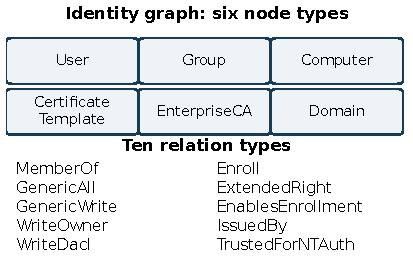
\includegraphics[width=\linewidth]{figures/revised_identity_schema.pdf}
\caption{Identity-graph abstraction: six node classes and ten relation types, matching Definition~\ref{def:identity_schema}. Relation instances depend on the directory export; not every type is exercised by every experiment.}
\label{fig:adcs_schema}
\end{figure}

\paragraph{Evaluated attack scope}
The live interventions test enrollee-supplied-subject policy and certificate mapping, with template mutation and restoration. These are ESC1-style issuance conditions with an ESC4-style modification step~\cite{schroeder2021certified}. Some archived filenames refer to other ESC scenarios, but those names do not establish successful exploitation. The synthetic learning predicate assumes resolved enrollment permissions; it does not validate ESC1--ESC15 coverage. CA-administration compromise, relay, issuance-policy group links and later ESC variants require separate policy and protocol evidence. They are outside the live coverage claim.

\subsection{Template Rollback and Snapshot Evidence}
Directory extraction tools such as BloodHound, SharpHound and Certipy provide configuration snapshots. Their scheduling is deployment-specific. Under temporal mutation-and-rollback attacks (such as ESC4 and ESC9), an attacker exploits transient write permissions to mutate a template, obtain a rogue certificate, and immediately roll back the attributes to their original configuration.

\begin{definition}[Static Snapshot Invariance under Rollback]
Let $t_0 < t_1 < t_2 < t_3$ denote the sequence of discrete timestamps in an attack execution lifecycle:
\begin{itemize}
    \item $t_0$: Pristine baseline state of directory $\mathcal{G}_{t_0}$.
    \item $t_1$: The attacker executes an LDAP modification adding \texttt{Enroll} permissions or setting \texttt{CT\_FLAG\_ENROLLEE\_SUPPLIES\_SUBJECT} on template $t$, yielding state $\mathcal{G}_{t_1}$.
    \item $t_2$: The attacker submits a certificate request and receives an issued certificate $\text{Cert}_{\text{admin}}$ valid for 1 year.
    \item $t_3$: The attacker rolls back the template modifications, restoring the directory attributes to their baseline state, yielding $\mathcal{G}_{t_3}$.
\end{itemize}
\end{definition}

\paragraph{Snapshot Indistinguishability and Evidence Scope}
For a projection restricted to configuration attributes restored by rollback, let $h_0$ and $h_1$ denote the digests before and during the mutation. The relevant equality is:
\begin{equation}
\fitmath{\begin{gathered}\text{SHA-256}(\mathcal{G}_{t_0}) = h_0\end{gathered}}
\end{equation}
\begin{equation}
\fitmath{\begin{gathered}\text{SHA-256}(\mathcal{G}_{t_1}) = h_1\end{gathered}}
\end{equation}
\begin{equation}
\fitmath{\begin{gathered}\text{SHA-256}(\mathcal{G}_{t_3}) = h_0\end{gathered}}
\end{equation}

This is a conditional indistinguishability argument for that projection, not evidence that the entire AD database is bit-identical. A detector restricted to this projection cannot distinguish the restored sequence from an unchanged configuration with the same projection. This is a statement about information available to the detector, not an empirical zero-recall estimate. The certificate can remain usable subject to validity, revocation, trust and account mapping. It does not imply that every directory or audit artifact disappears.

\subsection{Protocol Discontinuity: PKCS\#10 ASN.1 SAN Concealment and CA--KDC Logging Gap}
Collecting both CA and KDC Security events does not necessarily supply a shared certificate key. The relevant gap is missing certificate identity in the captured issuance event, rather than disjoint event-field names.

\paragraph{Captured event projections}
The selected issuance fields in Listing~\ref{lst:ca_event} are
\[\fitmath{\pi_{\mathrm{CA}}=\{\mathrm{RequestId},\mathrm{Requester},\mathrm{Subject},\mathrm{Attributes}\}.}\]
The certificate-bearing successful KDC record additionally exposes
\[\fitmath{\begin{gathered}
\pi_{\mathrm{KDC}}=\{\mathrm{TargetUserName},\mathrm{PreAuthType},\\
\mathrm{CertIssuerName},\mathrm{CertSerialNumber},\mathrm{CertThumbprint}\}.
\end{gathered}}\]
Neither Disposition nor SKID is shown in the selected 4887 payload. SKID and the other certificate identifiers used by the contract are obtained from the CA database export when available. Different field names alone say nothing about whether a join is possible: the issue is whether the captured values supply a shared, issuer-scoped certificate identity.

\paragraph{SAN fields in requests and audit records}
When an attacker requests a certificate with a rogue Subject Alternative Name (e.g., impersonating the Domain Administrator), the SAN attribute can be supplied through two distinct mechanisms:
\begin{enumerate}
    \item \textbf{Explicit RPC Attribute String:} Passed via the \texttt{Attributes} string parameter of \texttt{ICertRequest::Submit} (e.g., \texttt{"SAN:upn=Administrator@domain.local"}). In this configuration, the CA security log explicitly populates the \texttt{Attributes} field in Event ID 4887.
    \item \textbf{Raw PKCS\#10 ASN.1 Binary Extension:} Embedded directly within the cryptographic Certificate Signing Request (CSR) under the \texttt{szOID\_SUBJECT\_ALT\_NAME2} (\texttt{2.5.29.17}) extension attribute.
\end{enumerate}

Our forensic investigation of live archived GOAD event streams reveals that when an attacker employs the PKCS\#10 ASN.1 CSR extension (as executed natively by modern exploit tooling), the CA event log omits the SAN string entirely from the XML event payload:
\begin{lstlisting}[language=XML,caption={Selected fields from the independent 2019 enabled-condition capture: Security record 20539. The raw XML is retained in the artifact.},label=lst:ca_event]
<Event xmlns="http://schemas.microsoft.com/win/2004/08/events/event">
  <System>
    <Provider Name="Microsoft-Windows-Security-Auditing"/>
    <EventID>4887</EventID>
    <TimeCreated SystemTime="2026-11-10T10:53:51.393283900Z"/>
    <EventRecordID>20539</EventRecordID>
  </System>
  <EventData>
    <Data Name="RequestId">7</Data>
    <Data Name="Requester">Q1LAB\q1.enroller</Data>
    <Data Name="Subject">CN=q1.enroller</Data>
    <Data Name="Attributes">
CertificateTemplate:Q1Evidence
ccm:WIN-NA2FC16NO63.q1lab.test</Data>
  </EventData>
</Event>
\end{lstlisting}

Listing~\ref{lst:ca_event} contains a template and client-machine attribute, but no textual SAN UPN. The issued public certificate does contain the requested administrative SAN, and an exact-certificate successful KDC event independently checks its use. A query requiring a textual administrative SAN in this issuance event has no such input here; this is a concrete missing-field case, not a measured universal SIEM false-negative rate. The selected issuance event supplies a Request ID, whereas the certificate-bearing KDC record supplies issuer, serial, and thumbprint. SKID is optional CA-database enrichment, not a field demonstrated by this listing. The CA database export supplies the issuer-scoped bridge evaluated in Section~\ref{sec:evaluation}.

\section{Cryptographic Invariant Provenance Graph (CIPG)}
\label{sec:cipg_provenance}

To overcome the static snapshot blind spot and the CA--KDC schema discontinuity identified in Section~\ref{sec:threat_model}, we design the \textbf{Cryptographic Invariant Provenance Graph (CIPG)} (Figure~\ref{fig:neuro_symbolic_pipeline}). CIPG dynamically ingests raw Windows security audit event streams and CA transactional records, maintaining revisable lineage state across protocol layers. Provenance ingestion is independent of the optional graph classifier; neural-negative cases are not discarded.

\subsection{Multi-Source Provenance Ingestion and Entity Resolution}
CIPG processes heterogeneous audit streams across three disjoint operational layers:
\begin{enumerate}
    \item \textbf{Directory Service Audit Events (NTDS):} Monitored via Windows Security Event ID 5136 (\textit{Directory Service Object Modified}). Captures granular LDAP mutations on certificate templates, user objects, and access control lists, recording the modifying principal, target object GUID, modified attribute (e.g., \texttt{nTDSDSOptions}, \texttt{pKIExtendedKeyUsage}, \texttt{msPKI-Certificate-Name-Flag}), and operation type (Value Added / Value Deleted).
    \item \textbf{Certificate Authority Telemetry and CA DB Bridge:} Monitored via Event IDs 4886 (\textit{Certificate Request Received}) and 4887 (\textit{Certificate Issued}). To bridge missing shared certificate identifiers, CIPG queries the local CA transactional database using \texttt{certutil}, requesting the \texttt{RequestID}, \texttt{SerialNumber}, \texttt{SubjectKeyIdentifier}, and \texttt{CertificateHash} fields, or the raw CA RPC interface. This populates a persistent cryptographic tuple:
    \begin{equation}
\fitmath{\begin{gathered}\tau_{\text{crypto}} = \langle \text{Issuer}, \text{RequestID}, \text{SKID},\\  \text{SerialNumber}, \text{Thumbprint}_{\text{SHA1}} \rangle\end{gathered}}
\end{equation}
    \item \textbf{KDC Kerberos Pre-Authentication Events:} Monitored via Event ID 4768 (\textit{Kerberos Authentication Ticket Requested}). The successful-use reference accepts certificate pre-authentication types 15, 16 or 17 with a successful result. The highlighted live pilot uses type 16. It extracts the authenticating client name, domain target, certificate issuer CA, \texttt{CertSerialNumber}, and \texttt{CertThumbprint}; a nonzero result is recorded separately as a rejection, not a successful use.
\end{enumerate}

\begin{figure*}[ht]
\centering
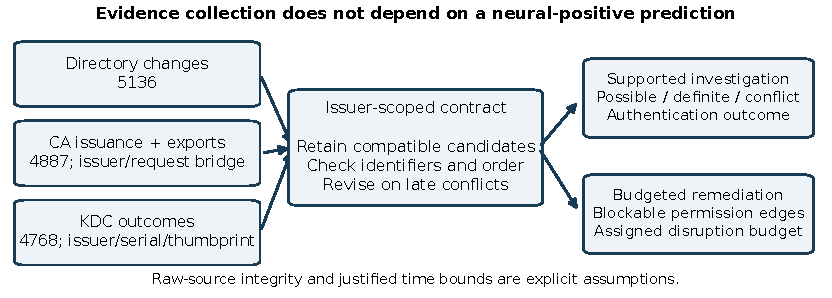
\includegraphics[width=\textwidth]{figures/revised_evidence_pipeline.pdf}
\caption{Evidence-first investigation. Directory changes, issuance records and KDC outcomes enter the issuer-scoped contract independently of optional learned screening. CA exports enrich identity; contradictory or incomplete evidence remains visible. Remediation uses supported explanations and its own budget model.}
\label{fig:neuro_symbolic_pipeline}
\end{figure*}

\subsection{Identity Decisions and Revision}
For an authentication observation $a$, the contract considers every captured issuance whose known identity fields are compatible with $a$. Request IDs are scoped by issuer when attaching CA exports. Serial equality is strong identity evidence only with issuer agreement; a shared thumbprint also supplies a strong certificate identifier. SKID alone is insufficient because a key may be reused. Missing fields remain unknown and cannot remove an otherwise compatible candidate to manufacture uniqueness.

A resolved identity requires one strongly identified candidate, agreement of all shared identifiers and no relevant source conflict. Multiple compatible candidates yield ambiguity; inconsistent attached observations yield conflicting evidence. Identity resolution and definite mutation overlap are separate outputs. The latter additionally requires justified operation order or time bounds. Late observations, export removal and conflicting evidence trigger reevaluation and can withdraw a resolved link. A guarded relational query implements these decisions on the same observations in Section~\ref{sec:evaluation}.

\subsection{Formal Cryptographic Invariants}
CIPG evaluates incoming event sequences against five formal behavioral and cryptographic invariants:

\begin{definition}[Invariant I: Two-Level Causal Invariant]
Let $e_{\text{mut}} \in \mathcal{E}_{\text{NTDS}}$ be a template ACL or attribute modification executed by principal $u_{\text{actor}}$, and let $e_{\text{req}} \in \mathcal{E}_{\text{CA}}$ be a certificate request submitted for template $t$. Invariant~I is satisfied if:
\begin{equation}
\fitmath{\begin{gathered}t(e_{\text{mut}}) < t(e_{\text{req}}) \\ \land\quad \text{TargetObject}(e_{\text{mut}}) = t \\ \land\quad \text{Requester}(e_{\text{req}}) \in \text{DelegatedPrincipals}(u_{\text{actor}})\end{gathered}}
\end{equation}
\end{definition}

\begin{definition}[Invariant II: Temporal-Order Sequence Invariant]
For any valid certificate lifecycle, the sequence of events must satisfy nondecreasing temporal progression:
\begin{equation}
\fitmath{t(e_{\text{mut}}) \le t(e_{\text{req}}) \le t(e_{\text{iss}}) \le t(e_{\text{auth}})}
\end{equation}
This progression refers to effective operations. An audit timestamp inconsistent with it can also arise from clock error, audit delay, or an incorrect event association; it does not alone establish spoofing or replay. When these assumptions cannot be justified, the implementation retains a possible explanation or reports inconsistent evidence.
\end{definition}

\begin{definition}[Invariant III: Principal Identity Discrepancy]
Let $R=\text{Requester}(e_{\text{req}})$ be the Windows security principal submitting the certificate enrollment request, and let $A=\text{TargetIdentity}(e_{\text{auth}})$ be the Kerberos client identity authenticating with the resulting certificate. An identity escalation violation occurs if:
\begin{equation}
\fitmath{R\neq A\quad\land\quad\text{PrivilegeLevel}(A)>\text{PrivilegeLevel}(R)}
\end{equation}
\end{definition}

\begin{definition}[Invariant IV: Rollback Reversal Detection]
Let $e_{\text{mut}}$ be an attribute modification on template $t$ at time $t_1$ adding an insecure flag $\text{attr}_{\text{vuln}}$, and let $e_{\text{roll}}$ be a subsequent modification at $t_3$ deleting $\text{attr}_{\text{vuln}}$. A rollback violation is triggered if:
\begin{equation}
\fitmath{\begin{gathered}\Delta t = t_3 - t_1 \le \tau_{\text{window}} \\ \land\quad \exists e_{\text{iss}} \in \mathcal{E}_{\text{CA}} \text{ s.t. } t_1 \le t(e_{\text{iss}}) \le t_3\end{gathered}}
\end{equation}
where $\tau_{\text{window}}$ is the maximum temporal attack window (set to 30 minutes in this model; it is not a measured enterprise policy).
\end{definition}

\subsection{Invariant V: Persistent Cryptographic Taint-Flow Automaton}
A same-actor or short-window rule can miss two important patterns: (i) \textbf{Split-Actor Collusion}, where Actor A mutates the template, Actor B requests the certificate, and Actor A rolls the template back; and (ii) \textbf{Dormant PKINIT Exploitation}, where the attacker delays Kerberos authentication by hours or days until the temporal correlation window $\tau_{\text{window}}$ has expired.

To retain certificate evidence beyond the immediate mutation window, we formalize the \textbf{Persistent Cryptographic Taint-Flow Automaton (Invariant~V)}. Its conclusions depend on captured identity evidence and retained state; it does not guarantee detection over an unbounded history:

\paragraph{Algorithm notation}
Let $\mathcal A_{\mathrm{mut}}$ contain \texttt{nTDSDSOptions}, \texttt{msPKI-Certificate-Name-Flag}, and \texttt{pKIExtendedKeyUsage}. The mutation map $\mathcal M$ stores the object GUID, actor, time and operation. The CA bridge $\mathcal B$ returns the certificate identifiers for an issuer/request pair. A taint entry retains these identifiers, requester, mutation actor and issuance time.

\begin{algorithm}[tbp]
\caption{CIPG certificate-lineage update}
\label{alg:invariant5}
\footnotesize
\begin{algorithmic}[1]
\Require Event stream $\mathcal S$, retained observations $\mathcal O$, current decisions $\mathcal D$
\For{each incoming event $e\in\mathcal S$}
 \State Add, replace or remove the affected observation in $\mathcal O$
 \State Attach exports by issuer/request; retain source conflicts
 \For{each affected certificate authentication $a$}
  \State Record failed or unknown outcomes separately
  \State Retain all compatible issuance candidates for successful use
  \State Check strong identity, ambiguity and conflicting evidence
  \State Evaluate possible/definite overlap under justified time constraints
  \State Compare with $\mathcal D[a]$; emit any revision or withdrawal
  \State Store the decision and its supporting observations
 \EndFor
\EndFor
\end{algorithmic}
\end{algorithm}


\paragraph{Mathematical Guarantees and Operational Concurrency Realities}
A serial number is scoped to its issuer~\cite{rfc5280}; SKID identifies a public key and can recur across distinct certificates. A thumbprint identifies certificate bytes, while an unauthenticated log field does not itself prove certificate possession or source integrity. The reference implementation requires all shared identity fields to agree and preserves compatible incompletely identified issuances, so missing fields cannot manufacture uniqueness. Late evidence can withdraw a previously resolved link. Retention enables delayed-use analysis only while the necessary observations remain available; no bounded-memory or irreversible-finality guarantee follows.

\paragraph{Bounded-time and source-fault reasoning}
For opening, issuance, and rollback intervals $O,I,R$, definite temporal overlap requires $O^{+}\le I^{-}$ and $I^{+}\le R^{-}$. Otherwise, a feasible overlap remains possible. An exact difference-constraint reference additionally accepts explicitly justified operation-order edges~\cite{dechter1991temporal,amarilli2019computing}; contradictory constraints yield an inconsistent-evidence answer. Cross-host record numbers do not supply those edges. This is an application of established temporal reasoning, with certificate-specific evidence requirements.

For a declared optional-export fault budget $k$, let $\mathcal{H}_k$ contain every deletion of at most $k$ CA bridge records. Candidate union over $\mathcal{H}_k$ preserves alternative explanations; a certain link must be resolved to the same issuance in every hypothesis. Abstaining hypotheses are retained, rather than removed to force agreement. If the true issuance is captured, raw issuance/KDC fields and time bounds are correct, and at most $k$ bridge records are faulty, deleting those faulty records leaves a hypothesis containing the true candidate. This is a conditional retention property, not a claim of certain resolution or robustness to compromised raw audit sources. The exhaustive implementation is a correctness reference with combinatorial cost, and source-level compromise can invalidate a record-level budget~\cite{elmagarmid2007duplicate,heinzl2026timestamps}.

The synthetic replay evaluates configured maintenance windows, background renewals and polling delays. Its collision counts describe that generated workload, not a universal arrival law. Section~\ref{sec:streaming_evaluation} gives the actual sampling scheme and separates matching-template collisions from the total renewal count.

\subsection{Graph Reduction and Meta-Node Compacting}
Repeated authentication observations can make a provenance graph costly to retain and query. The streaming CIPG implementation groups repeated events into meta-nodes:
\begin{equation}
\fitmath{\mathcal{C}: (v_{\text{event}}^{(1)}, v_{\text{event}}^{(2)}, \dots, v_{\text{event}}^{(m)}) \mapsto \mathcal{V}_{\text{meta}}}
\end{equation}
Whenever repetitive, non-mutating events share identical source principals, destination templates, and access control rights within a sliding window, CIPG collapses them into a single directed meta-edge annotated with frequency counters and temporal bounding intervals $[t_{\min}, t_{\max}]$. As quantified in Section~\ref{sec:evaluation}, this reduces graph storage overhead by \textbf{76.61\%} (compressing 10,182 raw elements to 2,382 compressed elements) while consuming only $6.91$~MB of memory at a sustained ingestion throughput of $13,192.4$~events/second.

\paragraph{Correlated optional sources and self-consistent false order}
Two explicit falsification controls test the boundaries of these guarantees. Six false bridge rows from one exporter exceed a two-record fault budget and produce a wrong certain link. A sufficient six-record reference retains the true candidate with 64 hypotheses; a whole-source deletion reference retains it with two hypotheses under the different assumption of at most one faulty failure domain. It abstains from certainty, and requires an explicitly supplied source partition rather than treating file copies as independent origins. This is a failure-model comparison, not equal-budget accuracy superiority.

A second control supplies true times $o=0$, $c=1$, $i=2$ inside declared bounds $[0,3]$, then fabricates the jointly consistent order $o\le i\le c$. The temporal solver returns definite overlap although the latent history has none. Thus consistency checking cannot authenticate the order channel. The controlled orchestrator is an additional trusted source in our pilot; its truth assumption cannot be replaced by the mere absence of contradictory constraints.

\section{Disruption-Budgeted Sequential Interdiction}
\label{sec:game_theoretic}

A supported certificate-use explanation can identify permissions for hardening, but revocation has operational costs. We evaluate a separate graph-remediation task: choose blockable permission edges whose removal disconnects specified source--target pairs under an assigned budget. The utility counts disconnected pairs; it does not depend on an attacker's choice among surviving paths. Accordingly, the evaluated method is a sequential interdiction heuristic, not a computed strategic equilibrium.

\subsection{Budgeted Pair-Disconnection Objective}
Let $E_b\subseteq\mathcal E$ be the blockable edges and $\mathcal Q=\{(s_i,t_i)\}_{i=1}^{k}$ the queried compromise pairs. Define $D(C)$ as the number of pairs disconnected after removing $C\subseteq E_b$.

\paragraph{Heterogeneous Operational Revocation Costs}
In enterprise Active Directory environments, revoking different permission types imposes vastly unequal operational disruption on legitimate business workflows. We assign heterogeneous cost functions $c: \mathcal{E} \to \mathbb{R}^+$ as model parameters, without a measured mapping to enterprise impact:
\begin{equation}
\fitmath{c(e)=\begin{cases}
 c_{\mathrm{group}}\in[2.8,3.8], & \psi(e)=\mathrm{MemberOf},\\
 c_{\mathrm{acl}}\in[2.0,3.0], & \psi(e)\in\{\mathrm{GenericAll},\mathrm{WriteDacl}\},\\
 c_{\mathrm{choke}}\in[1.0,1.4], & \begin{gathered}\psi(e)\in\{\mathrm{Enroll},\\ \mathrm{EnablesEnrollment}\}.\end{gathered}
\end{cases}}
\end{equation}
The assigned disruption labels are high for changes to user-role workflows, medium for changes to administrative synchronization, and low for template-enrollment reconfiguration.


The evaluated objective is
\begin{equation}
\fitmath{\max_{C\subseteq E_b}D(C),\qquad
D(C)=\sum_{i=1}^{k}\mathbb I[t_i\notin\operatorname{Reach}_{\mathcal G\setminus C}(s_i)],}
\end{equation}
\begin{equation}
\fitmath{\text{subject to}\quad\sum_{e\in C}c(e)\le B_{\mathrm{ops}}.}
\label{eq:budget_constraint}
\end{equation}
The small-instance audit uses cost as the exact solver's tie-break among equal-disconnection cuts. The sequential heuristic uses costs in candidate ranking; neither choice represents a measured administrator utility. Classical interdiction models provide the broader optimization context~\cite{wood1993interdiction,israeli2002shortest}.

\subsection{Computational Complexity: NP-Hardness of Multi-Principal Access Interdiction}
We show that finding the optimal edge revocation strategy to neutralize multiple compromise paths under budget constraints is intractable.

\begin{theorem}[NP-Hardness of Multi-Principal Access Interdiction]
\label{thm:nphardness}
Let $\mathcal{G} = (\mathcal{V}, \mathcal{E})$ be a directed identity multigraph with positive binary-encoded rational edge revocation costs and budget, and let $\mathcal{P}_{\text{forbidden}} = \{(s_1, t_1), \dots, (s_k, t_k)\}$ be $k \ge 3$ source-target compromise pairs, with $k$ part of the input. Pairs may share endpoints; no endpoint-disjoint restriction is asserted. The Multi-Principal Access Interdiction (MPAI) problem, which decides whether there exists $E_{\text{cut}} \subseteq \mathcal{E}$ with $\sum_{e \in E_{\text{cut}}} c(e) \le B_{\text{ops}}$ such that all paths in $\mathcal{P}_{\text{forbidden}}$ are severed, is NP-complete.
\end{theorem}

\begin{proof}
We establish membership in NP and provide a polynomial-time reduction from the NP-complete \textbf{Directed Multiway Cut} problem~\cite{garg1994multiway}.

\paragraph{Part 1: Membership in NP.}
Given a candidate cut set $E_{\text{cut}} \subseteq \mathcal{E}$:
\begin{enumerate}
    \item We compute $\sum_{e \in E_{\text{cut}}} c(e)$ in $\mathcal{O}(|E_{\text{cut}}|)$ time and verify the budget condition (\ref{eq:budget_constraint}).
    \item We construct the residual graph $\mathcal{G}' = (\mathcal{V}, \mathcal{E} \setminus E_{\text{cut}})$ in $\mathcal{O}(|\mathcal{V}| + |\mathcal{E}|)$ time.
    \item For each $(s_i, t_i) \in \mathcal{P}_{\text{forbidden}}$, we run Breadth-First Search (BFS) in $\mathcal{G}'$ starting from $s_i$ to verify that $t_i$ is unreachable in $\mathcal{O}(k \cdot (|\mathcal{V}| + |\mathcal{E}|))$ time.
\end{enumerate}
Because all checks execute in deterministic polynomial time, $\text{MPAI} \in \text{NP}$.

\paragraph{Part 2: Reduction from Directed Multiway Cut.}
Directed Multiway Cut takes a directed graph $H=(V_H,E_H)$, positive rational edge costs $w$, terminals $X=\{x_1,\ldots,x_q\}$, and budget $W$, and asks whether a cut of cost at most $W$ removes every path between distinct terminals. This known NP-hard problem is a special source of interdiction instances; the complexity classification is not a new graph-theoretic discovery.

Retain every vertex and edge of $H$, with its original cost. For each terminal $x_i$, add distinct source and target copies $s_i,t_i$, with connector edges $(s_i,x_i)$ and $(x_i,t_i)$ of cost $W+1$. Set
\begin{equation}
\fitmath{\mathcal{P}_{\mathrm{forbidden}}=\{(s_i,t_j):i\ne j\},\qquad B_{\mathrm{ops}}=W.}
\end{equation}
No budget-feasible cut can remove a connector. A path from $s_i$ to $t_j$ therefore exists exactly when a path from $x_i$ to $x_j$ remains in $H$, including paths passing through other terminals. Consequently, feasible cuts correspond with identical cost in both directions. The construction adds $2q$ vertices, $2q$ edges, and $q(q-1)$ forbidden pairs, and has polynomial encoding length. Together with polynomial verification of a candidate cut and rational budget, this proves NP-completeness of the stated general pair problem. It does not establish a new hardness result for a fixed pair count or for a particular restricted AD graph family.
\end{proof}

\subsection{Adaptive and Static Greedy Heuristics}
We compare simple degree-based and cost-aware static shortest-path-participation heuristics. The latter computes initial path participation divided by assigned edge cost once, so it already accounts for cost. Its limitation is the fixed ranking: earlier cuts can make later candidates redundant, and new shortest paths can change which permissions matter. The adaptive policy recomputes this information after each chosen cut. Degree-only ranking is a distinct baseline and need not have the same cost sensitivity. These are implemented research comparators rather than measured deployments of an industrial remediation product.

The evaluated \textbf{adaptive sequential policy} recomputes active shortest paths and candidate marginal pair-disconnection gains after each cut. It can select low-cost enrollment edges when they lie on relevant paths. Removing a candidate temporarily must preserve every edge attribute when the candidate is restored; relation and immutability metadata affect subsequent scoring. The implementation supplies no global optimum or approximation guarantee. Exact small-instance comparisons quantify its observed suboptimality.

\subsection{Operational Edge Immutability ($E_b \subsetneq E$) and Provenance-Cone Scalability}
As considered in AD graph-hardening work~\cite{goel2024hardening}, not all permissions can be revoked without breaking production workflows. A realistic fraction of permissions represents operational dependencies (e.g., core domain controllers, long-lived service accounts, or administrative replication pipelines) where IT administrators enforce $e \notin E_b$ (\texttt{blockable = False}). Because of these immutable operational corridors, the metadata-preserving adaptive rerun reports $98.5 \pm 4.0\%$ disconnected pairs at $B_{\text{ops}}=24$ (vs. $97.6 \pm 6.5\%$ for static greedy). The eight-test Holm analysis in Section~\ref{sec:evaluation} gives adjusted $p=0.25$ for both budget-24 procedures, leaving a measured mean residual of approximately $1.5\%$ on those synthetic instances. This is not a proof that the residual is irreducible or that CIPG is its only possible defense.

We evaluate a path-preserving projection on identical pairs in Section~\ref{sec:evaluation}. Every pair endpoint and every vertex on a requested source--target path is retained, with unchanged edge attributes. This permits a meaningful comparison of the same reachability objective, including projection overhead, without treating a smaller query set as an algorithmic speedup.

\paragraph{Exact small-instance audit}
Exhaustive feasible cuts on 30 seven-node, twelve-edge graphs at two budgets produce 60 cases. The metadata-preserving adaptive heuristic matches the optimal severed-pair count in 43/60 cases, compared with 21/60 for static greedy, and has a maximum gap of two pairs. This is a finite-instance comparison, not an optimality guarantee. Appendix~\ref{sec:artifact_corrections} records the attribute-restoration control, including the uncorrected implementation's 46/60 optimum matches.

\section{Empirical Evaluation and Live Cyber-Range Benchmarks}
\label{sec:evaluation}

We separate certificate identity, temporal attribution and graph hardening. The primary questions are:
\begin{itemize}
\item \textbf{RQ1 (Attribution):} Which certificate-specific links and mutation overlaps are supported under incomplete identifiers, optional-source faults and time uncertainty?
\item \textbf{RQ2 (Collection and retention):} What costs are measured for replay, offline reasoning and periodic collection, and which costs remain unmeasured?
\item \textbf{RQ3 (Remediation):} What pair-disconnection values, cut counts and optimality gaps occur under assigned costs and immutable edges?
\end{itemize}
The optional GNN diagnostic is reported in Appendix~\ref{sec:graph_evaluation}. It is not evidence of certificate exploitation or a prerequisite for the live evaluation. Unless otherwise stated, dispersions are population standard deviations of the finite evaluated seeds, folds or graphs; paired tests use the saved per-graph observations.

\subsection{Experimental Setup}
\paragraph{Synthetic Identity Graphs} The class-balanced static benchmark uses 700 class-balanced synthetic identity graphs. Additional graph sizes are used in the separate scalability experiments. Neither the class proportions nor the graph generator constitute a measured enterprise distribution. The matched gating audit uses the existing two-step implementations with fixed source snapshots and separately recorded training, validation, and test inputs.

\paragraph{Controlled Windows testbeds} We use a virtualized Game of Active Directory (GOAD) cyber-range. Inventory of the restored DC and CA identifies Windows Server 2016 Standard Evaluation, build 14393. The two nodes are:
\begin{itemize}
    \item \texttt{DC03} (\texttt{essos.local}): Active Directory Domain Controller, Kerberos KDC, and LDAP directory.
    \item \texttt{SRV03} (\texttt{braavos.essos.local}): Certificate Authority running Microsoft Active Directory Certificate Services.
\end{itemize}
The split-actor case uses domain accounts \texttt{ESSOS\textbackslash khal.drogo} and \texttt{ESSOS\textbackslash viserys.targaryen}. Original disk images were read-only; execution used writable overlays. The capture pipeline runs non-interactively, while restoring the old VM images required console-assisted recovery. A second, independently provisioned forest uses Windows Server 2019 build 17763.4974, its own CA and ordinary enroller, and host-generated SHA-256-signed requests. This measured 2023 patch level is not described as a current patched configuration.

\subsection{RQ1 and RQ2: Provenance Evidence and Collection Cost}
\label{sec:streaming_evaluation}
We separate seven archived trace files, one new outcome-checked Windows case, a synthetic attribution confirmation study, and the earlier $10,182$-event trace-driven synthetic stress stream. Their outcome definitions and evidence levels differ; scenario filenames are not independent success labels.

\begin{table}[tbp]
\centering
\caption{Audit of Seven Archived GOAD Files: 586 Raw Events. Linkage concerns the captured certificate issuance-to-use chain. Attack recall is not established for any file.}
\label{tab:live_traces}
\evidencetable
\setlength{\tabcolsep}{2pt}
\begin{tabular}{@{}>{\raggedright\arraybackslash}p{.32\linewidth}r>{\raggedright\arraybackslash}p{.51\linewidth}@{}}
\toprule
Scenario & Events & Captured linkage \\
\midrule
Normal enrollment & 89 & No consistent captured issuance \\
ESC4 rollback & 90 & No consistent captured issuance \\
ESC6 CA flag scenario & 172 & KDC failure result \texttt{0x42} \\
ESC9 UPN swap & 94 & No consistent captured issuance \\
ASN.1 SAN concealment & 88 & No consistent captured issuance \\
Admin typo rollback & 6 & No certificate-use observation \\
Split-actor scenario & 47 & Resolved observed linkage \\
\bottomrule
\end{tabular}
\end{table}

\begin{table}[tbp]
\centering
\caption{Trace-Driven Synthetic Streaming Benchmark ($10,182$ Events, 48 Generated Attack Instances, 50 Simulated Maintenance Windows). The table measures the streaming implementation, not the constraint reference.}
\label{tab:cipg_stress}
\evidencetable
\setlength{\tabcolsep}{2pt}
\begin{tabular}{@{}>{\raggedright\arraybackslash}p{.30\linewidth}*{5}{>{\centering\arraybackslash}p{.12\linewidth}}@{}}
\toprule
Pipeline & \textbf{Prec.} & \textbf{Recall} & \textbf{F1} & \makecell{Maint.\\FPR} & \makecell{Event\\FPR} \\
\midrule
Snapshot rollback & 19.35\% & 25.00\% & 21.82\% & 100.0\% (50/50) & 0.49\% \\
CA event 4887 & 88.24\% & 58.33\% & 70.16\% & 0.00\% (0/50) & 0.00\% \\
\makecell[l]{CIPG, default\\$\Delta_{\text{poll}}=5$ s} & \textbf{92.16\%} & \textbf{97.92\%} & \textbf{94.95\%} & \textbf{8.00\% (4/50)} & \textbf{0.0395\%} \\
\makecell[l]{CIPG, fast\\$\Delta_{\text{poll}}=1$ s} & \textbf{92.31\%} & \textbf{100.00\%} & \textbf{96.00\%} & \textbf{8.00\% (4/50)} & \textbf{0.0395\%} \\
\bottomrule
\end{tabular}
\end{table}

\begin{table}[tbp]
\centering
\caption{2D Sensitivity Matrix: Precision above recall (\%) across Correlation Horizon ($\Delta t$) and CA Jet DB Polling Lag ($\Delta_{\text{poll}}$).}
\label{tab:sensitivity_matrix}
\evidencetable
\setlength{\tabcolsep}{2pt}
\begin{tabular}{@{}lcccc@{}}
\toprule
\makecell{Window (s)\\FPR (\%)} & \makecell{Poll\\1 s} & \makecell{Poll\\5 s} & \makecell{Poll\\15 s} & \makecell{Poll\\60 s} \\
\midrule
\makecell[l]{10\\0.0} & \makecell{100.0\%\\100.0\%} & \makecell{100.0\%\\97.92\%} & \makecell{100.0\%\\89.58\%} & \makecell{100.0\%\\89.58\%} \\
\makecell[l]{30\\6.0} & \makecell{94.12\%\\100.0\%} & \makecell{94.00\%\\97.92\%} & \makecell{93.48\%\\89.58\%} & \makecell{93.48\%\\89.58\%} \\
\makecell[l]{60\\8.0} & \makecell{92.31\%\\100.0\%} & \makecell{92.16\%\\97.92\%} & \makecell{91.49\%\\89.58\%} & \makecell{91.49\%\\89.58\%} \\
\makecell[l]{300\\8.0} & \makecell{92.31\%\\100.0\%} & \makecell{92.16\%\\97.92\%} & \makecell{91.49\%\\89.58\%} & \makecell{91.49\%\\89.58\%} \\
\makecell[l]{900\\8.0} & \makecell{92.31\%\\100.0\%} & \makecell{92.16\%\\97.92\%} & \makecell{91.49\%\\89.58\%} & \makecell{91.49\%\\89.58\%} \\
\bottomrule
\end{tabular}
\end{table}

\paragraph{Collection delay and attribution trade-offs}
As documented in Table~\ref{tab:cipg_stress} and Table~\ref{tab:sensitivity_matrix}, in the configured synthetic CA/KDC workload, operational performance is governed by two orthogonal systems dimensions:
\begin{itemize}
    \item \textbf{Correlation horizon and collisions:} The generator fixes 2,000 renewal arrivals uniformly over the simulated duration $T$; it does not sample an unconditional 2,000-per-hour Poisson process. Each renewal selects a maintenance template with probability $0.055$, uniformly among 15 templates; otherwise it selects the machine template. For one maintenance template and a horizon $\Delta\le T$, the simplified matching-arrival probability is $1-(1-0.055\Delta/(15T))^{2000}$, before any additional principal or detector conditions. Thus an aggregate arrival count cannot be substituted for the rate of matching template/principal events. In the seeded realization, the sensitivity query reports 0/50 collisions at 10~s, 3/50 at 30~s and 4/50 from 60~s onward. These are observed finite-workload counts, not estimates of collision-free production operation. Generated maintenance durations lie in $[10,35]$~s. The plateau concerns the retained workload and query; it is not a universal Poisson law.
    \item \textbf{CA Database Polling Lag ($\Delta_{\text{poll}}$) vs. False Negatives:} Because KDC Event 4768 omits SubjectKeyIdentifier (SKID), linking these selected issuance and authentication records requires the CA database or an equivalent captured certificate-identity bridge. When an attacker's PKINIT execution delay $\delta_{\text{pkinit}} \sim \text{LogNormal}(1.2, 0.8)$ executes before the next polling tick ($t_{\text{auth}} + \Delta_{\text{watermark}} < t_{\text{poll}}$), the join keys remain un-enriched at evaluation time, producing unresolved links at the fixed evaluation deadline. At $\Delta_{\text{poll}} = 1.0\text{s}$, CIPG achieves $100.00\%$ recall ($48/48$). At default $\Delta_{\text{poll}} = 5.0\text{s}$, CIPG achieves $97.92\%$ recall ($47/48$). At $\Delta_{\text{poll}} \in \{15\text{s}, 60\text{s}\}$, rapid attacks beat the polling cycle, resulting in $89.58\%$ recall ($43/48$).
\end{itemize}

\paragraph{Ingestion Throughput and Memory Profiling}
On the finite replay workload:
\begin{itemize}
    \item \textbf{Throughput:} The saved streaming benchmark reports \textbf{13,192.4 events/second} (771.81~ms) on the configured synthetic stream. This excludes a demonstrated end-to-end Windows collection/deployment pipeline and is not a throughput measurement of the constraint reference reasoners.
    \item \textbf{Memory Footprint:} The streaming result reports \textbf{6.91 MB}. A finite-run measurement does not establish bounded retained memory as the certificate history grows.
    \item \textbf{Meta-Node Compression:} Meta-node compacting collapsed 10,182 raw elements into 2,382 compressed elements, achieving a \textbf{76.61\% reduction in graph size} in the benchmark's repeated-event representation.
\end{itemize}

\paragraph{Outcome-checked split-actor pilot}
The split-actor capture contains 49 selected raw Security records. CA request 25 and issuance record 65102 identify the exact public certificate subsequently observed in successful KDC record 168295 (status zero, PKINIT type 16, domain Administrator SID ending in 500). The issued certificate and exported private key were checked for identity before use; the original template flag was restored. A failed first capture is preserved and excluded. The configured delay was 14 seconds after the rollback step, not 24 hours. This establishes one controlled outcome, rather than an attack recall estimate.

The pre-capture clock-offset bracket fails a consistency check: the rollback audit timestamp precedes the host's rollback invocation under that constant-offset model. Point-time and assumed-error outputs therefore cannot establish guaranteed audit-time attribution. Separately, the frozen synchronous orchestrator records mutation completion before submission and retrieval of the exact issued certificate before rollback. Difference constraints over that additional operation-order channel establish controlled issuance between those operations without aligning the Windows audit clocks. Removing any one of the five required order edges returns a merely possible overlap. This does not establish when the CA consumed template policy, rule out every intervening mutation, or prove that the changed flag was necessary for issuance.

\paragraph{Locally frozen confirmation and component studies}
The constraint reference was frozen before a five-seed confirmation run containing 5,400 cases and 27,000 method/case predictions. Table~\ref{tab:lineage_confirmation} reports the 2,000 variable-size histories separately from repeated logical challenges and forged-log controls. Compared with the conjunctive point-time baseline, the prototype makes fewer definitive claims: it resolves 55.82\% rather than 74.56\% of true observed links, retaining 99.06\% in possible sets. It recovers 107 of 539 true mutation overlaps definitively with zero false overlap claims, versus 310 correct and 51 false claims for the point baseline. This is a coverage/certainty trade-off, not universal superiority. All 200 internally consistent forged-record controls defeat every method; truthful raw sources remain an explicit premise.

A separate source-hash-frozen factorial study uses 2,700 identity histories and 1,800 temporal histories from an independent component generator. The temporal solver agrees with 3,600 independently enumerated query answers. With a fully observed additional order channel, it recovers all 138 true overlaps in 300 histories; interval boxes recover 53 and point time recovers 112 with 11 false claims (Table~\ref{tab:order_component}). All 900 intentionally contradictory-order controls are rejected by the order-aware method. Complete observation is a designed upper-bound condition, not a measured enterprise sensor rate.

The bridge study tests zero to two faulty export records and fault budgets $k\in\{0,1,2\}$ (Table~\ref{tab:bridge_component}). The $k=2$ reference retains all 2,180 true links as candidates, but resolves only 602 certainly. Discarding all optional exports retains the same true links and resolves 1,757 certainly in this grid. The repair method therefore has no demonstrated advantage over that ablation here. Its exhaustive 49,800 hypotheses expose the cost of the fault contract and motivate testing independently corroborated enrichment, rather than claiming a solved robust-attribution problem. The artifact verifier checks latent labels, counts, hashes, temporal oracle answers, and within-budget retention; it does not prove optimality of repair candidate sets. None of these local comparators is an execution of Splunk or HADES.

\paragraph{Published-rule field-requirement replay}
We also execute a SQLite candidate-association proxy for the SAN/principal conditions in Splunk's published ESC1 analytic~\cite{splunk2026esc1}. This is not a Splunk runtime reproduction: scheduling, macros, default join-result truncation, and multivalue behavior are outside the proxy. Seven archived files plus the new pilot contain only one issuance satisfying the textual SAN/UPN prerequisite, in the ESC6 file. Literal principal association returns no pair; an explicitly separate short-name normalization adaptation returns one pair whose KDC status is the failure value \texttt{0x42}. The successful split-actor pilot lacks the textual SAN prerequisite. These results expose required evidence and normalization choices; they do not estimate Splunk's attack precision or recall or compare unlike task outputs as exact certificate linkage.

% Generated from hash-verified saved research artifacts; do not hand-edit.
\begin{table}[tbp]
\centering
\caption{Confirmation on 2,000 synthetic histories: 1,804 true observed links and 539 true mutation overlaps. Link coverage is a percentage; overlap entries are edge counts. These are attribution outcomes, not exploit detection rates.}
\label{tab:lineage_confirmation}
\evidencetable
\begin{tabular}{lrrrr}
\toprule
Method & \makecell{Definite\\links (\%)} & \makecell{Possible\\links (\%)} & \makecell{True\\overlap} & \makecell{False\\overlap} \\
\midrule
Identifier OR & 91.69 & 91.69 & 374 & 175 \\
Issuer--serial & 62.86 & 62.86 & 265 & 88 \\
Conjunctive, 300 s & 47.67 & 47.67 & 196 & 34 \\
Conjunctive, point & 74.56 & 74.56 & 310 & 51 \\
\makecell[l]{CIPG constraint\\reference} & 55.82 & 99.06 & 107 & 0 \\
\bottomrule
\end{tabular}
\end{table}
\begin{table}[tbp]
\centering
\caption{Temporal component study, 300 histories per observation rate. The order-aware method receives an additional explicit sensor channel; no cross-host ordering is inferred from record numbers. Each row is evaluated on the same cases as the other methods at that rate.}
\label{tab:order_component}
\evidencetable
\begin{tabular}{rlrrr}
\toprule
\makecell{Order\\rate} & Method & \makecell{True\\overlaps} & Recovered & \makecell{False\\claims} \\
\midrule
0 & Point time & 122 & 93 & 18 \\
0 & Interval boxes & 122 & 54 & 0 \\
0 & \makecell[l]{Intervals +\\observed order} & 122 & 54 & 0 \\
0.5 & Point time & 148 & 104 & 12 \\
0.5 & Interval boxes & 148 & 59 & 0 \\
0.5 & \makecell[l]{Intervals +\\observed order} & 148 & 88 & 0 \\
1 & Point time & 138 & 112 & 11 \\
1 & Interval boxes & 138 & 53 & 0 \\
1 & \makecell[l]{Intervals +\\observed order} & 138 & 138 & 0 \\
\bottomrule
\end{tabular}
\end{table}
\begin{table}[tbp]
\centering
\caption{Bridge-fault component study: 2,700 histories, 2,180 successful observed links. Fault counts range from zero to two; budgets below the true count include outside-assumption controls. Candidate retention and certain-link coverage are reported separately.}
\label{tab:bridge_component}
\evidencetable
\begin{tabular}{lrrrr}
\toprule
Method & \makecell{Retained\\true links} & \makecell{Certain\\true links} & \makecell{Wrong\\certain} & Hypotheses \\
\midrule
$k=0$ & 1440 & 721 & 0 & 2700 \\
$k=1$ & 1811 & 602 & 0 & 15300 \\
$k=2$ & 2180 & 602 & 0 & 49800 \\
\makecell[l]{Ignore optional\\exports} & 2180 & 1757 & 0 & 2700 \\
\bottomrule
\end{tabular}
\end{table}
\begin{table}[tbp]
\centering
\caption{Matched policy interventions: three blocks per OS and three certificate uses per condition. The 2019 build is 17763.4974. Signed administrative CSR/key pairs are matched within blocks. ESC1 and risky EKU measure template configuration, not attack intent.}
\label{tab:paired_live_policy}
\evidencetable
\begin{tabular}{llrrrrr}
\toprule
OS & Condition & Trials & Self & Admin & ESC1 & \makecell{Risky\\EKU} \\
\midrule
2016 & \makecell[l]{Baseline/admin\\request} & 3 & 3 & 0 & 0 & 0 \\
2016 & \makecell[l]{Subject bit\\enabled} & 3 & 0 & 3 & 3 & 3 \\
2016 & \makecell[l]{Rollback before\\request} & 3 & 3 & 0 & 0 & 0 \\
2016 & \makecell[l]{Legitimate self\\request} & 3 & 3 & 0 & 3 & 3 \\
2019 & \makecell[l]{Baseline/admin\\request} & 3 & 3 & 0 & 0 & 0 \\
2019 & \makecell[l]{Subject bit\\enabled} & 3 & 0 & 3 & 3 & 3 \\
2019 & \makecell[l]{Rollback before\\request} & 3 & 3 & 0 & 0 & 0 \\
2019 & \makecell[l]{Legitimate self\\request} & 3 & 3 & 0 & 3 & 3 \\
\bottomrule
\end{tabular}
\end{table}


\paragraph{Repeated fixed-request policy interventions and executed external rules}
We extend the initial pilot with a locally frozen 12-trial matrix and three repeated intervention blocks (Table~\ref{tab:paired_live_policy}). Within each block, baseline, enabled, and rollback-before-request conditions reuse identical signed CSR bytes and the same public key. Only the enrollee-supplied-subject bit changes; recorded template DACL, EKU, approval, signature, and OID fields remain equal. CA cache refresh and low-privilege RPC readiness checks are applied consistently. The enabled condition produces three exact-certificate Administrator authentications. Baseline and rollback-before-request conditions each produce three ordinary-user authentications, despite requesting the same administrative SAN. Three legitimate self-enrollments also authenticate as the ordinary user. All 12 outcomes are checked against public certificate bytes, CA database/4887 evidence, successful 4768 outcomes, target SID/name/domain, mutation evidence, and restoration. These controlled contrasts support necessity of the tested bit for the privileged outcome under the recorded conditions; they do not turn temporal overlap alone into a causal explanation.

The collector binds the verified held key to the exact issued certificate and rejects unrelated keys. The Windows 2016 fixed requests have the observed SHA-1 signature algorithm; independent Windows 2019 requests use SHA-256. Infrastructure failures and excluded collection attempts are documented in Appendix~\ref{sec:artifact_corrections}.

Certipy 5.0.4 is executed against LDAP for each assigned configuration using its DC-only mode. Three unmodified upstream Sigma rules~\cite{sigma2026rules} are compiled by pySigma 2.1.0~\cite{pysigma210}/SQLite backend 2.1.1~\cite{pysigma_sqlite211} and executed on the captured event fields. Template-load events 4898 supply the actual tested-template configuration. Both Certipy's ESC1 finding and Sigma's risky-EKU predicate identify all three enabled administrative conditions and all three enabled legitimate-self conditions, with no tested-template match in baseline or rollback-before-request conditions. That agreement concerns risky configuration, not malicious intent: legitimate self-enrollment does not become an attack false positive merely because its template remains risky. Sigma matches on other loaded templates are retained separately. The machine-account rule has no matching human-account target. This is an actual external-rule/tool execution, separate from the earlier Splunk semantic proxy and from a full SIEM or HADES deployment.

\paragraph{Independent forest replication and measured collection cost}
We repeat the four-condition matrix in a newly provisioned \texttt{q1lab.test} forest, with its own \texttt{Q1-Evidence-CA}, ordinary \texttt{q1.enroller} account, separate template, and host-generated SHA-256-signed CSRs. All 12 exact-certificate outcomes are verified: three enabled-condition Administrator uses and nine self-uses. Three matched signed-request/policy blocks reproduce the controlled contrast. Some restoration value-addition events are absent despite successful write responses and restored readback; certificate-use validation and complete mutation-audit history are therefore reported separately. The measured build, 17763.4974, predates current strong-binding enforcement updates~\cite{microsoft2025strongbinding}. Excluded setup attempts do not enter the policy or detection denominator (Appendix~\ref{sec:artifact_corrections}).

On the independent captures, raw template names and CA database template OIDs initially disagree, causing the identity reference to abstain in all 12 cases. Adding the collected directory object's explicit OID/name mapping resolves all 12 identities, with three privileged SID divergences and nine nonprivileged outcomes. Certificate/CSR bytes and adjudicator labels remain excluded from inference. The mapping is a development adjustment; the prospective transfer cohort below uses the frozen detector. Actual Certipy/Sigma configuration-risk results repeat the Windows 2016 pattern in the independent forest.

The median recorded command envelope is 50.91~s per trial on the two-node 2016 setup and 32.14~s on the single-node independent 2019 setup. Ten offline identity-inference repetitions per captured trial give medians across trials of 10.99~ms and 9.18~ms, respectively. Python-traced peak allocations are approximately 1.74~MB and 1.50~MB at the median. These measurements describe the captured experiment and offline inference; they do not measure continuous polling delay, host RSS, or enterprise authentication interference.

\paragraph{Current-patch request forms and post-rollback observation}
We update the independent forest using signed Microsoft packages to Windows Server 2019 build 17763.9376 (October 2026 security update KB5126651~\cite{microsoft2026october2019}). Post-reboot inventory verifies the installed build, no pending reboot, running CA/KDC services, an ordinary enroller, and enabled Defender. No binding-compatibility override is introduced. Two locally frozen 12-trial protocols repeat the four conditions with UPN-only and UPN-plus-SID-URL requests. Administrative requests reuse identical signed CSR bytes and keys within each block and request form; keys are not matched across forms. The SID URL follows the documented Microsoft mapping format~\cite{microsoft2025pkcasid}. All conditions in these matrices include restored template readback, CA refresh, RPC readiness and actual Certipy enumeration before authentication. These additional controls differ from the older-build workflow, so the old/new contrast is not an isolated patch-only experiment.

\input{generated/current_patch_evidence}

The UPN-only matrix yields six verified ordinary-user authentications and six certificate-bound KDC rejections: all three enabled administrative requests and all three enabled legitimate-self requests are rejected. The six rejected public certificates lack the security SID extension and match KDC System event 39 by serial and thumbprint. Baseline and rollback-before-request certificates contain the enroller SID extension and authenticate as that user. With a matching SID URL, all 12 outcomes authenticate: three enabled administrative uses and nine self-uses. The enabled certificates contain the requested SID URLs and lack the security SID extension. Three fixed-request/policy blocks support the conditional enabling-bit contrast for this form; no such privileged-use contrast is observed for UPN-only requests. These observations accord with the documented distinction between weak names and strong certificate mapping~\cite{microsoft2025strongbinding,microsoft2025pkcasid}; adding a SID URL is not a new exploitation technique.

Actual Certipy and Sigma executions retain the same pre-request risky-configuration pattern in both matrices. All 24 post-rollback Certipy enumerations cease flagging ESC1 on the tested template, including the three cases that subsequently authenticate as Administrator. This demonstrates that restored configuration and the later usability of an issued certificate are different questions. It does not establish attack intent or superiority over a provenance system given equivalent certificate evidence. The unchanged identity reference links all 18 successful current-patch authentications, including three privileged SID divergences, without certificate/CSR bytes or adjudicator labels as inference inputs. Rejected authentications are outside this successful-use linkage denominator.

An adjudication audit identifies a collector defect: an empty System-log query prevented the following CA database export in 18 trials. A separately recorded later read-only CA snapshot supplies only those missing exports in ephemeral verification views; all original captures and manifests remain unchanged. Matching public certificate bytes, CA rows, trial issuance events and KDC evidence then resolves all 24 outcomes. This later snapshot does not establish historical template state or repair the audit-clock model. A live empty-query control validates the collector correction before the restored lab is shut down. Across the four final matrices, 48 trials therefore provide 42 successful exact-certificate authentications, including nine administrative uses, and six exact-certificate rejections.

\paragraph{Equal-input relational realization and revision}
We execute two SQLite correlators on the same canonical observations as the identity reference. A strong conjunctive join resolves a unique strong, nonconflicting match; a guarded query also retains incomplete candidates and relevant conflicts. All event intervals are projected to $[0,0]$, with no mutation windows, so this experiment concerns identity and revisions rather than temporal attribution. Across 1,470 seeded histories, the guarded query and reference agree at all 5,423 evaluated prefixes. Independent set-based verification checks 16,269 prediction rows and 450 saved latent random-history labels. Both methods retract 225 provisional resolved links during shuffled delivery and bridge removal/reinsertion. This establishes relational realizability of the contract; the query is our implementation in SQLite, not an execution of HADES or Splunk.

\input{generated/gap_closure_evidence}

The main 1,410-case group includes 60 chronology-negative controls, which produce wrong terminal claims in every identity-only method because time was erased. A separate 60 consistently forged-source controls also fool every method. The guarded contract retains more true candidates but resolves fewer correct links than the strong join on this challenge. We therefore do not claim unique reasoning power or universal superiority over a competent relational implementation. Candidate completeness, temporal evidence and source truth remain separate requirements.

\paragraph{Prospective concurrent transfer to a new forest}
Before collection, we freeze the unchanged identity detector and a new workload protocol. A writable child of the updated Windows image is demoted and reprovisioned as \texttt{q1transfer.test}, with a fresh domain SID, hostname, CA, two templates and two ordinary enrollers. The seed and original disk mounts remain read-only. This transfers identity namespaces and workload conditions while sharing the Windows image family. Six batches each issue four certificates through overlapping enrollment command envelopes. Each enroller reuses one RSA key across its certificates, with identical signed request bytes within each enroller/target group. These are repeated issuances with reused keys, not a Windows renewal-protocol experiment.

All 24 distinct public certificates match their CSR keys, CA issuance and successful KDC outcomes: 20 self-uses and four administrative uses. Every batch has four overlapping submission command envelopes; that does not prove simultaneous CA execution. All 24 leaf signatures verify under the separately captured public CA certificate, whose current NTAuth membership is observed. The frozen detector links all 24 successful uses, including four privileged SID divergences. A reporting fix leaves mutation-history fields unvalidated for the transfer condition names; certificate-use criteria and labels are unchanged. Actual Certipy/Sigma findings are counted in 12 distinct template/batch/enroller units, since two certificate cases share each enumeration. All 12 postrollback enumerations cease flagging tested-template ESC1. The six batch exports contain 4,544 Security events, including process creation/termination, explicit credentials and service-ticket events. They are not full Sysmon/file/socket provenance for an end-to-end PIDS comparison.

\paragraph{Paired collection and authentication-envelope pilot}
A separately frozen pilot compares periodic collection with an idle collector in three seeded arm orders on the restored transfer forest. Each arm performs eight legitimate certificate authentications at a three-second target start period. Polling targets two seconds, exports incremental Security records and the CA database, updates the identity reference and retains checkpoints. Independent public-certificate/KDC checks validate all 48 measured authentications. Median authentication process envelopes increase by 48.6, 80.0 and 100.3~ms in the three pairs. These include Certipy startup and network work; they are not packet-level KDC latency or a production interference bound.

The 33 polling iterations have per-arm median collection-plus-reasoning envelopes of 1.586--1.659~s. Sampled Python collector RSS ranges from 56.5 to 59.5~MiB across arms, excluding Certipy children and the Windows VM. Periodic reference state grows from 30 seeded records to 37 records, with a 16,000-byte final checkpoint in each polling arm. This short pilot does not establish bounded lifetime retention or maximum sustainable throughput. Outcome verification waits until after the measured interval, preserving the authentication timing denominator. Excluded collection attempts are described in Appendix~\ref{sec:artifact_corrections}.

\subsection{RQ3: Budgeted Sequential Interdiction}
We evaluated the adaptive sequential policy against three standard remediation baselines across 30 generated identity graphs:
\begin{enumerate}
    \item \textbf{Random Cut:} Selects arbitrary reachable edges within budget.
    \item \textbf{Degree Centrality:} Selects edges incident to the highest-degree nodes.
    \item \textbf{Static Greedy:} Ranks participation in initially selected shortest paths once, divided by assigned revocation cost, then cuts feasible edges in that order.
    \item \textbf{Adaptive sequential:} Applies the sequential reachability heuristic to the interdiction formulation under heterogeneous operational disruption costs and operational edge immutability ($E_b \subsetneq E$).
\end{enumerate}

\input{generated/interdiction_recheck_evidence}

\begin{figure}[tbp]
\centering
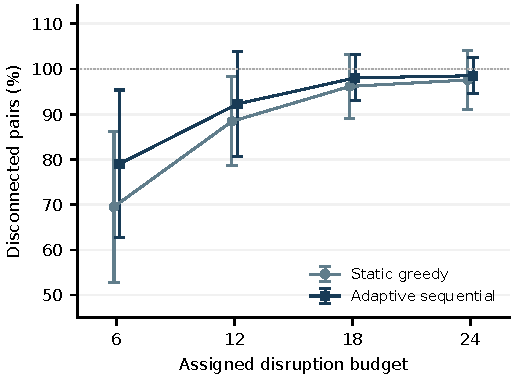
\includegraphics[width=\linewidth]{figures/revised_interdiction_results.pdf}
\caption{Measured disconnected-pair percentages on 30 generated graphs. Error bars show population SD across graphs. Horizontal values are assigned cost budgets. These are fixed-budget outcomes, not convergence trajectories.}
\label{fig:stackelberg_convergence}
\end{figure}

\paragraph{Operational Immutability Plateau and the Runtime Defense Residual}
In enterprise networks, a realistic fraction of directory edges represents immutable operational dependencies ($E_b \subsetneq E$). As shown in Table~\ref{tab:stackelberg_results} and Figure~\ref{fig:stackelberg_convergence}, proactive graph interdiction achieves \textbf{$98.5 \pm 4.0\%$} paths severed at $B_{\text{ops}}=24$ (vs. $97.6 \pm 6.5\%$ for Static Greedy).
This experiment leaves a mean residual of approximately $1.5\%$ under the selected graph instances, budgets, and non-blockable edges. It does not prove that every enterprise has an unavoidable residual of that size or that a different feasible policy cannot disconnect all modeled paths. Runtime monitoring is complementary to the evaluated hardening policies.

\paragraph{Paired tests and multiple comparisons}
Independent adjacency-list checks validate all 120 budget/cut outcomes and 11,100 reachability queries. Table~\ref{tab:stackelberg_results} compares adaptive and static greedy on the same 30 graphs using a paired $t$-test and exact signed-rank enumeration. The eight-test Holm family covers four budgets and two procedures~\cite{holm1979simple}. Budget 6 survives both procedures; budget 18 survives only exact signed rank (adjusted $p=0.02344$, paired-$t$ adjusted $p=0.05138$). At budget 24, only five paired differences are nonzero and all are positive. Exact enumeration over $2^5=32$ sign assignments gives raw $p=0.0625$; the mean gain is 0.94 percentage points. Both adjusted budget-24 values are $p=0.25$. The measurements therefore do not support a significant budget-24 difference. Ranks use exact rational disconnection fractions and omit zero differences. This is a descriptive synthetic-graph analysis, not evidence of enterprise operational superiority.

\paragraph{Revoked-edge count}
Under $B_{\text{ops}} = 24$, Static Greedy revokes an average of \textbf{10.9 edges} ($10.9 \pm 0.9$), under the assigned heterogeneous costs. The saved summary does not measure the resulting business-workflow disruption. The metadata-preserving adaptive rerun revokes an average of \textbf{5.7 edges} ($5.7 \pm 2.3$), a \textbf{47.7\% reduction in revoked-edge count}. The disruption weights are assigned model parameters; actual administrator effort and business disruption were not measured.

\input{generated/projection_evidence}

\paragraph{Scalability via Provenance-Cone Guidance}
We implement a path-preserving projection. For every requested pair $(s,t)$, retain the intersection of vertices reachable from $s$ and vertices that can reach $t$, together with every pair endpoint. Every original $s$--$t$ path is retained, so subsequent removal of any retained edge subset preserves that pair's reachability answer. Edge costs, relations and immutability are copied unchanged, and initially unconnected endpoints remain represented. Intersecting any full-graph cut with the retained edge set removes no requested-path effect and cannot increase its nonnegative cost, so the optimal budgeted pair-disconnection value is also preserved. A heuristic's selected cut can still depend on its search order. Shared endpoint closures are computed once per distinct endpoint.

The equal-query benchmark retains all pairs, uses the same sequential heuristic on full and projected graphs, and includes projection cost (Table~\ref{tab:scalability_bench}). At 5,000 actual nodes and 325 queried pairs, 874--890 nodes remain. Across fifteen alternating-order timing pairs, the median per-run ratio is $7.54\times$, with observed range $6.62$--$8.99\times$, and severed-pair outcomes agree in every run. The median full and projection-inclusive times are 3,448.15~ms and 439.29~ms; their ratio need not equal the median of individual ratios. This controlled result does not supply an optimality or enterprise workload guarantee.

\section{Discussion and Limitations}
\label{sec:discussion}
\subsection{Collection Cost and Deployment Scope}
The synthetic replay reports 13,192.4 events/sec and 6.91 MB on a fixed stream. Those measurements do not establish zero interference with domain authentication, bounded history storage, or end-to-end CA polling cost. The lineage reference recomputes retained evidence, and the fault-budget reference enumerates deletion hypotheses. The recorded live command envelopes and offline inference timings quantify two parts of this cost: median recorded trial envelopes are 50.91~s and 32.14~s in the two environments, while median offline identity reasoning is 10.99~ms and 9.18~ms. A three-pair collection pilot measures periodic export/reference updates and verifies 48 legitimate authentications. The paired median client process-envelope increases are 48.6--100.3~ms, with sampled Python collector RSS of 56.5--59.5~MiB, excluding children and the VM. This quantifies a short isolated-lab workload; continuous high-load operation, lifetime retention and production interference remain unestablished.

\subsection{Hybrid Identity Evaluation}
The experiments cover on-premises ADCS and KDC records. Extending the evidence contract to Microsoft Entra ID would require additional identity-mapping and audit-source assumptions. Cross-tenant tokens and synchronization-account compromise are outside the evaluated workload. They should be treated as separate validation tasks before making claims about hybrid identity protection.

\subsection{Threats to Validity and Limitations}
We distinguish the following threats to validity and experimental limitations:
\begin{enumerate}
    \item \textbf{Evidence Scale and Label Validity:} The archive's scenario names do not establish seven successful attacks. Four final fixed-request matrices supply 42 successful exact-certificate authentications and six certificate-bound rejections, with nine privileged uses and matched self-use controls. A prospective transfer cohort adds 24 distinct certificates, including four further privileged uses: the combined primary studies contain 72 certificate cases, 66 successful uses and six rejections. The transfer cohort has new identity namespaces and concurrent multi-template activity but shares the Windows image family. They establish controlled outcomes, not enterprise prevalence. Independent Windows 2019 builds 17763.4974 and 17763.9376 are measured. Current-patch controls reveal request-form differences, but the additional post-rollback workflow prevents attributing every old/new difference solely to the update. Eighteen missing contemporaneous CA exports are explicitly supplemented by a later read-only snapshot; original captures remain intact. Original source images remain read-only.
    \item \textbf{Static Model and Generator Validity:} The matched audit checks reachable-path labels and checks 6,000 checkpoint predictions. Repeated training/validation archetypes, fixed first-step transforms, hand-initialized projections, and the distinction between feature-channel and bilinear gating restrict what its numbers establish. A separate literal bilinear study removes those implementation and repeated-whole-input problems with trainable encoders and typed family-disjoint splits. Both literal bilinear and additive attention still miss all 450 long-path positives per arm, without a classification advantage for gating. A verifier restricted to neural positives cannot repair these misses, and symbolic label agreement is not independent Windows ground truth.
    \item \textbf{Parametric Disruption Costs vs. Interactive Administrator Feedback:} In the budgeted interdiction model, operational disruption costs $c(e)$ are assigned parametrically according to relation type ($c(\text{MemberOf}) \in [2.8, 3.8], c(\text{GenericAll}) \in [2.0, 3.0], c(\text{Enroll}) \in [1.0, 1.4]$) and operational edge immutability constraints ($E_b \subsetneq E$). In production enterprise deployments, operational criticality is context-sensitive and evolving. The exact small-instance audit gives concrete optimum comparisons rather than a universal heuristic guarantee. A metadata-preserving rerun also checks all 120 original graph/budget instances; it changes nine objective outcomes and 24 cut counts. The primary table and revoked-edge comparison use full edge-attribute restoration (Appendix~\ref{sec:artifact_corrections}). Eliciting and validating administrator-assigned costs requires a separate evaluation; the graph-hardening study~\cite{goel2024hardening} is not cited as evidence of such preference elicitation.
    \item \textbf{Trust, Time, and Necessary Causation:} Candidate retention under a bridge fault budget assumes correct raw issuance/KDC records and captured true issuance. Consistently forged raw histories defeat the methods, while faults exceeding the declared budget invalidate its retention guarantee. A counterexample shows that self-consistent false order can also produce a wrong definite overlap. A grouped-source reference handles the six-record correlated-export control under an explicit one-source assumption, which differs from a record budget. The operation-order pilot uses the controlled orchestrator as an additional trusted source and does not repair the failed Windows audit-clock model. Temporal overlap alone does not establish necessity. The matched CSR/key interventions support a conditional contrast under the recorded policy fields and controlled CA refresh, while unobserved concurrent changes and missing restoration audit events remain distinct evidence concerns.
\end{enumerate}

\section{Conclusion}
\label{sec:conclusion}
CertGraph links certificate issuance and use under an explicit issuer-scoped evidence contract. Its live evaluation verifies 66 successful certificate authentications and six certificate-bound rejections, including 13 administrative uses. The current-patch controls show why a restored template scan and a certificate-use investigation answer different questions. The identity contract can also be implemented using guarded SQL; the evaluated contribution concerns its security requirements and evidence handling rather than a unique reasoning primitive.

The graph-learning results do not establish a classification advantage for bilinear gating. Both matched literal models miss the tested long-path positives, so a verifier that examines only neural-positive cases remains incomplete for this workload. The remediation experiments also show heuristic optimality gaps and budget-dependent differences from greedy selection. Larger deployments require separate measurements of collection cost, retained history and administrator-assigned disruption costs. The present results support these specific conclusions within the recorded laboratory and generator conditions.

\section*{Author Contributions}
\noindent\textbf{Md.~Hasan~Shahriar}: Conceptualization, Methodology, Software, Formal Analysis, Investigation, Writing -- Original Draft, Visualization, Project Administration.
\textbf{Taufiq~Biswas}: Validation, Data Curation, Formal Analysis, Writing -- Review \& Editing.
\textbf{Md.~Ramim~Hossain}: Validation, Resources, Investigation, Writing -- Review \& Editing.

\section*{Conflicts of Interest}
\noindent The authors declare that they have no known competing financial interests or personal relationships that could have appeared to influence the work reported in this paper.

\section*{Funding}
\noindent This research received no specific grant from any funding agency.

\section*{Ethics and Dual-Use Considerations}
\noindent The reported interventions concern isolated, researcher-controlled Windows forests and laboratory accounts. They test certificate abuse and permission changes solely to assess defensive evidence and remediation. Original disk images were retained read-only, and writable overlays were used for the experiments. No production organization or unsuspecting user was part of the evaluated workload. Credential-bearing material, private keys and reusable authentication tokens are excluded from the review artifact. The review package retains synthetic controls, verification code and derived results; the original live evidence remains in controlled storage.

\section*{Data and Code Availability}
\noindent The supplementary review artifact contains the synthetic study inputs, source snapshots, verification results and manuscript evidence tables described in this paper. The artifact README identifies omitted credential-bearing laboratory material and the resulting reproduction limits. The project repository is \url{https://github.com/hasanshahriar32/CertGraph-CIPG}; a persistent, versioned public archive of this revision has not yet been deposited. No archive DOI is claimed.


\appendices
\section{Auxiliary Graph Screening: Formulation and Limits}
\label{sec:certgraph_arch}

This appendix describes an optional screening experiment. It does not supply the paper's provenance correctness claim or a gate that restricts evidence collection. The matched study in Appendix~\ref{sec:graph_evaluation} finds no classification advantage for bilinear gating.

\subsection{Heterogeneous Graph Attention Network (HetGAT)}
Following graph-learning formulations~\cite{scarselli2008graph,wu2021survey}, CertGraph employs a multi-relational graph attention network. Let $\mathbf{x}_v \in \mathbb{R}^{d_{\phi(v)}}$ denote the initial feature vector of entity $v \in \mathcal{V}$. Vertices are first projected into a shared hidden space of dimension $d$:
\begin{equation}
\fitmath{\mathbf{h}_v^{(0)} = \text{ReLU} \left( \mathbf{W}_{\phi(v)}^{(0)} \mathbf{x}_v + \mathbf{b}_{\phi(v)}^{(0)} \right)}
\end{equation}
where $\mathbf{W}_{\phi(v)}^{(0)} \in \mathbb{R}^{d \times d_{\phi(v)}}$ is a type-specific linear projection matrix.

At each layer $l \in \{1, \dots, L\}$, message passing aggregates relational representations across incoming edges $\mathcal{N}_r(v) = \{u \in \mathcal{V} \mid (u, v) \in \mathcal{E}, \psi(u, v) = r\}$:
\begin{equation}
\fitmath{\mathbf{h}_v^{(l)} = \sigma \left( \sum_{r \in \mathcal{R}_{\text{in}}(\phi(v))} \sum_{u \in \mathcal{N}_r(v)} \alpha_{vu}^{(l)} \mathbf{W}_r^{(l)} \mathbf{h}_u^{(l-1)} \right)}
\end{equation}
where $\mathbf{W}_r^{(l)} \in \mathbb{R}^{d \times d}$ is the relation-specific weight transformation for relation $r \in \mathcal{T}_E$, and $\sigma(\cdot)$ denotes the ELU activation function. The relational attention coefficient $\alpha_{vu}^{(l)}$ assigns dynamic importance to edge $(u, v)$ under relation $r$:
\begin{equation}
\fitmath{\begin{gathered}
\alpha_{vu}^{(l)}=\frac{\exp(z_{vu}^{(l)})}{\sum_{k\in\mathcal N_r(v)}\exp(z_{vk}^{(l)})},\\
z_{vu}^{(l)}=\operatorname{LeakyReLU}\!\left(\mathbf a_r^\top
\begin{bmatrix}\mathbf W_r^{(l)}\mathbf h_v^{(l-1)}\\ \mathbf W_r^{(l)}\mathbf h_u^{(l-1)}\end{bmatrix}\right).
\end{gathered}}
\end{equation}
where $\mathbf{a}_r \in \mathbb{R}^{2d}$ is the parameterized attention vector for relation $r$, and $\|$ denotes vector concatenation.

\subsection{Target-Feature Dependence and Residual Sensitivity}
\label{thm:theorem1}
Absence of an explicit self-loop does not imply independence from target features. Writing the first-layer pre-activation as $s_v=\sum_{r,u}\alpha_{vu}W_rh_u^{(0)}$, its derivative includes
\begin{equation}
\fitmath{\frac{\partial s_v}{\partial h_v^{(0)}}=
\sum_{r,u}(W_rh_u^{(0)})\frac{\partial\alpha_{vu}}{\partial h_v^{(0)}}.}
\end{equation}
For the target-dependent attention defined above, this term need not vanish. It vanishes for a coefficient-independent variant with independent node inputs and no self-loop; only that restricted variant erases the target's own first-layer input. An empty incoming neighborhood yields zero only when there is no bias and the activation maps zero to zero.

For a residual model in a common $d$-dimensional hidden space, let $P_v=W_{\mathrm{skip}}^{(L)}\cdots W_{\mathrm{skip}}^{(1)}$ and let $J_{\mathrm{other}}$ collect every non-skip derivative, including derivatives through attention. At a differentiable input,
\begin{equation}
\fitmath{\begin{gathered}
J_v=\frac{\partial\widetilde h_v^{(L)}}{\partial h_v^{(0)}}=P_v+J_{\mathrm{other}},\\
\sigma_{\min}(J_v)\ge\prod_{l=1}^{L}\sigma_{\min}(W_{\mathrm{skip}}^{(l)})
-\|J_{\mathrm{other}}\|_2.
\end{gathered}}
\end{equation}
This follows from the singular-value perturbation inequality and the product bound for square matrices. A positive lower bound requires the skip product to dominate the other derivative. It does not guarantee sensitivity to raw features before the type projection, nor validate every attention architecture. We use it as a conditional diagnostic, not a theorem about shortcut elimination.

\subsection{Shortcut Behavior and Bilinear Gating}
While the analysis in Appendix~\ref{sec:certgraph_arch} gives a conditional sensitivity bound for additive residual skips ($\tilde{\mathbf{h}}_v^{(l)} = \mathbf{h}_v^{(l)} + \mathbf{W}_{\text{skip}}^{(l)} \tilde{\mathbf{h}}_v^{(l-1)}$), empirical testing reveals a secondary failure mode: \textit{inductive shortcut collapse}.

\paragraph{The Shortcut Memorization Failure}
Because certificate template attributes (e.g., \texttt{CT\_FLAG\_ENROLLEE\_SUPPLIES\_SUBJECT} $= 1$ and Client Authentication EKU $= 1$) are strongly correlated with positive escalation labels in synthetic training distributions, additive skip connections provide a route by which the readout can emphasize template attributes. An attribute-dominated shortcut can take the form:
\begin{equation}
\fitmath{\hat{y}_t = \text{MLP}(\tilde{\mathbf{h}}_t^{(L)}) \approx \text{MLP} \left( \prod_{k=1}^L \mathbf{W}_{\text{skip}}^{(k)} \mathbf{h}_t^{(0)} \right)}
\end{equation}
When the trained model is evaluated against \textbf{adversarial hard negatives}—templates that possess vulnerable attribute flags but reside in disconnected graph components or require mandatory manager approval—standard additive-skip GNNs memorize the flag pattern and classify them as vulnerable, showing poor agreement on the canonical generator. The matched audit in Appendix~\ref{sec:graph_evaluation} checks its reachable-path labels and separates augmentation from implementation differences.

\paragraph{Multiplicative Bilinear Reachability Gating (\texttt{CertGraph-Gated}):}
To test whether learned compatibility changes this behavior, we condition messages on a learned bilinear compatibility gate. The division between learned scoring and symbolic checking follows a broader neuro-symbolic design~\cite{garcez2023neurosymbolic}. Exact reachability is checked separately by the existing symbolic verification step; the learned gate alone is not a Boolean authorization predicate. We formulate the \textbf{Multiplicative Bilinear Reachability Gate}:
\begin{equation}
\fitmath{\mathbf{g}_{uv}^{(l)} = \sigma \left( \mathbf{h}_u^{(l-1)\top} \mathbf{W}_g^{(l)} \mathbf{h}_v^{(l-1)} + b_g^{(l)} \right)}
\end{equation}
where $\mathbf{W}_g^{(l)} \in \mathbb{R}^{d \times d}$ is a bilinear interaction matrix, $b_g^{(l)} \in \mathbb{R}$ is a scalar bias, and $\sigma(\cdot)$ is the sigmoid function mapping to $(0, 1)$.

The gated message vector $\mathbf{m}_{vu}^{(l)}$ and state update are defined as:
\begin{equation}
\fitmath{\begin{gathered}\mathbf{m}_{vu}^{(l)} = \mathbf{g}_{uv}^{(l)} \odot \left( \mathbf{W}_r^{(l)} \mathbf{h}_u^{(l-1)} \right)\end{gathered}}
\end{equation}
\begin{equation}
\fitmath{\begin{gathered}\mathbf{h}_v^{(l)} = \sigma \left( \sum_{r \in \mathcal{R}_{\text{in}}(\phi(v))} \sum_{u \in \mathcal{N}_r(v)} \alpha_{vu}^{(l)} \mathbf{m}_{vu}^{(l)} \right)\\ \quad+\mathbf{g}_{vv}^{(l)} \odot \left( \mathbf{W}_{\text{skip}}^{(l)} \mathbf{h}_v^{(l-1)} \right)\end{gathered}}
\end{equation}
where $\odot$ denotes the element-wise Hadamard product.

\begin{proposition}[Conditional Attenuation by Multiplicative Gating]
For a bounded transformed neighbor message, if its scalar gate tends to zero, multiplicative attenuation gives:
\begin{equation}
\fitmath{\lim_{\mathbf{g}_{uv} \to 0} \mathbf{m}_{vu}^{(l)} = \mathbf{0}}
\end{equation}
Disconnection alone does not imply this gate limit: with zero embeddings and zero bias, the sigmoid gate equals $1/2$. Other residual paths or classifier biases can also produce a positive output. The attenuation statement therefore does not prove universal elimination of shortcuts. The feature-channel numerical implementation uses a feature-channel gate rather than this literal scorer. We implement a separate two-layer, four-head realization of the displayed bilinear edge and self-skip equations and evaluate it with identical-initialization additive controls and matched augmentation (Table~\ref{tab:literal_bilinear}). All relevant parameter families are trainable through autograd. The two implementations have identical held-out classifications in the matched study, and both miss the positive long-path cases. This validates an auditable realization of the formulation, rather than a universal shortcut-elimination or authorization guarantee. A second-tier verifier must process unresolved and out-of-horizon cases, including neural negatives, if it is to recover those observed misses.
\end{proposition}

\section{Auxiliary Graph-Learning Evaluation}
\label{sec:graph_evaluation}

\subsection{In-Distribution Ablations and Perturbation Asymmetry}
We first distinguish the class-balanced generator from the attribution and live-policy experiments. Their labels, model implementations, and observation units differ.

\paragraph{Skip-connection ablation}
The saved five-fold artifact reports Macro-F1 $0.9986 \pm 0.0029$ with skips and $0.4768 \pm 0.0239$ without skips. Recomputing the paired statistic from the five saved fold values gives $t=46.245$, $p=1.308\times10^{-6}$, and four degrees of freedom. The dispersions are population standard deviations across these folds. Shared training data and generator assumptions limit interpretation of this descriptive comparison. This ablation is not an empirical validation of the conditional derivative analysis in Appendix~\ref{sec:certgraph_arch}.

\paragraph{Class Proportions and Probability Interpretation}
The static experiments reported here are generator-based classification studies. Their balanced labels do not establish a 96\% enterprise safe base rate, and their softmax scores are not calibrated probabilities of real-world compromise. We retain probabilities and selected checkpoints in the matched audit so that classification errors can be checked independently.

\paragraph{Perturbation Asymmetry and Simple Comparators}
The saved robustness artifact gives Macro-F1 $0.9479$ after 30\% edge perturbation, compared with $0.8965$ and $0.7709$ after 5\% and 10\% feature perturbation. This sensitivity pattern motivates testing structural counterfactuals; it does not prove that every prediction ignores topology. A separately verified, previously saved three-seed ESC13 abstraction also favors simple graph-count models over the existing GNN on its IID cases. Its symbolic reference defines the labels, so its perfect agreement is a consistency result rather than independent exploit validation.

\subsection{Generalization and Hard-Negative Diagnostics}
A source audit identifies two problems with interpreting the original-label $41/63$ safe-label agreement as a general hard-negative detection result. Ten ``deep horizon'' cases retain a membership path to an allowed enrollment group and therefore are positive under a transitive effective-permission interpretation. The stored 22 disagreements are eight administrator-only write cases, four deny-write cases, seven benign OID links, and three deep OID links; the disagreements are reported using their stored categories. The canonical generator also repeats inputs across training and validation. These original-label counts are retained in the artifact but do not establish independent-case specificity or a binomial confidence interval.

We therefore freeze and execute a matched $2\times2$ diagnostic: additive versus feature-channel-gated implementations, each with counterfactual augmentation probability zero or 0.3, across three independently selected seeds. Model equations, propagation depth, and original artifacts remain unchanged. Each seed evaluates 250 opposite-label families, with membership depths 0, 1, 2, 4, and 8, randomized node order, and matched configuration features. Positive members retain reachable enrollment; negative members either restrict enrollment to the administrator or add a reachable explicit deny. Queue traversal and Boolean closure independently agree on all test labels under this stated ESC1 permission abstraction. CA trust and resolved permissions are assumed; Windows exploitability is not the label definition.

\input{generated/gating_evidence}

The gate gives zero false positives but misses all 450 positive cases at depths 2, 4, and 8 across the three seeds. Adding the same augmentation to the additive implementation improves its pooled accuracy from 50\% to 71.67\%, compared with the gate's 70\%. Thus the audit does not establish superiority of gating over an augmentation-matched comparator. First-step membership transforms are fixed in these existing NumPy implementations, and their feature-channel gate is $\sigma(W_{\mathrm{gate}}\mu_{\mathrm{reach}}+b)$, rather than a literal implementation of the general bilinear edge scorer in Section~\ref{sec:certgraph_arch}. Initialization also differs between implementations. These distinctions prevent attributing the entire contrast to a bilinear operation.

Only 22 unique training inputs occur per seed, with 21 also present in validation. Consequently, validation selection in this diagnostic is not an independent-distribution generalization test. All 6,000 saved test predictions are reproduced from saved checkpoints, and their labels and aggregates are checked independently. A symbolic second tier must also examine unresolved or out-of-horizon cases: verifying only neural-positive candidates cannot recover these observed neural false negatives.

\paragraph{Literal bilinear realization and family-disjoint validation}
We address the implementation mismatch with a separate literal realization of the bilinear edge and self-skip equations: two relational-attention layers, four heads, 32 hidden channels, type-specific input projection, and fully trainable encoder, attention, skip, and gate parameters. The binary readout evaluates the stated ESC1 resolved-permission predicate, not observed Windows compromise. Additive and gated arms start with identical parameter values and receive matched augmentation. Neither symbolic closure nor outcome labels enter the forward pass. Gradient, node-relabeling, and padding checks validate implementation properties; the feature-channel implementations are retained separately.

The family-disjoint generator constructs varied reachable and unreachable membership branches and paired allow/deny interventions. For each of three independently selected seeds, 300 training and 100 validation families are separated from 150 families in each of IID, long-path, and larger-background test cohorts. Typed five-round Weisfeiler--Lehman input hashes and family IDs are disjoint across splits within a seed. This conservatively excludes isomorphic whole inputs under the encoded roles and edge types, without claiming disjoint local motifs. Long-path positive enrollment chains have membership depth 2, 4, or 8. The larger-background cohort adds isolated nodes to different generated families; it is not a matched causal estimate of graph-size effects or enterprise-scale generalization.

% Generated from verified literal bilinear checkpoint predictions.
\begin{table}[tbp]
\centering
\caption{Literal two-layer attention: mean accuracy (\%) $\pm$ population SD over three seeds. Each test cohort contains 150 paired families per seed; initialization and augmentation are matched.}
\label{tab:literal_bilinear}
\evidencetable
\begin{tabular}{llrrr}
\toprule
Model & Aug. & IID & \makecell{Long\\paths} & \makecell{Larger\\background} \\
\midrule
\makecell[l]{Additive\\attention} & 0 & $86.00 \pm 1.78$ & $50.00 \pm 0.00$ & $87.00 \pm 0.82$ \\
\makecell[l]{Additive\\attention} & 0.3 & $86.00 \pm 1.78$ & $50.00 \pm 0.00$ & $87.00 \pm 0.82$ \\
\makecell[l]{Bilinear\\attention} & 0 & $86.00 \pm 1.78$ & $50.00 \pm 0.00$ & $87.00 \pm 0.82$ \\
\makecell[l]{Bilinear\\attention} & 0.3 & $86.00 \pm 1.78$ & $50.00 \pm 0.00$ & $87.00 \pm 0.82$ \\
\bottomrule
\end{tabular}
\end{table}


Independent NetworkX reachability checks all 5,100 saved case labels, and checkpoint inference reproduces all 10,800 held-out predictions. The literal bilinear and additive models have identical classifications in every matched arm: IID accuracy averages $86.00\%\pm1.79\%$, larger-background accuracy $87.00\%\pm0.82\%$, and long-path accuracy 50\%. In each arm, all 450 positive long-path cases are missed. Some IID negatives also require deny-membership reasoning beyond the local horizon; 126 pooled false positives remain. Probability scores differ, but their reported calibration errors concern these synthetic cohorts only. This closes the literal-implementation and repeated-whole-input gaps while failing to establish classification superiority for bilinear gating. Exact verification of unresolved cases remains necessary under the stated permission contract.


\section{Artifact Corrections and Excluded Runs}
\label{sec:artifact_corrections}
The retained artifact distinguishes source captures, adjudication views and derived results. Exclusions are methodological, not additional negative policy outcomes:
\begin{itemize}
\item A first split-actor capture failed and is excluded; the outcome-checked pilot has a 14-second post-rollback delay, not a 24-hour delay.
\item A development matrix contains two RPC failures among twelve attempts. A fixed-request collector stops on a pending-request-store key-binding failure. These attempts are separate from the four final matrices and their 48 outcome-checked cases.
\item An independent-forest setup with a four-hour clock difference is excluded. The accepted 2019 inventory is build 17763.4974 before update and 17763.9376 afterward; the restored GOAD nodes are Windows Server 2016 build 14393.
\item An empty System-log query suppresses eighteen contemporaneous CA exports. A later read-only CA snapshot supplies these exports only in separate adjudication views. It does not reconstruct missing historical template state or correct the failed audit-clock model.
\item A collection-pilot attempt exports final outcome evidence too early. The accepted timing study waits for outcome verification after the measured interval and validates all 48 authentications.
\item In the interdiction scoring control, temporary edge deletion restores only cost and loses other attributes. Restoring every attribute changes nine of 120 disconnection outcomes and 24 cut counts. The primary table uses full restoration. In the separate 60-case exact audit, the uncorrected control matches the optimum in 46 cases, versus 43 for full restoration; a correctness fix is not claimed as an accuracy improvement.
\item A depth-limited cone timing compares different queried pairs and uses 4,551 actual nodes for a nominal 5,000-node graph. Its $1,246.3\times$ ratio is excluded from the speedup claim. The reported projection benchmark retains identical queried pairs and includes construction cost.
\end{itemize}
The hard-negative diagnostic contains $41/63$ safe-label agreements under its original labels; it is not a zero-agreement result. Ten deep-horizon cases are positive under transitive enrollment. Appendix~\ref{sec:graph_evaluation} reports corrected labels, repeated-input limitations and separate family-disjoint evaluation rather than using this count as independent specificity.


\bibliography{references}

\end{document}
